\begin{appendix}

\section{Mask R-CNN: training history and qualitative results}
\label{app:maskrcnn}

Figure~\ref{fig:curves} shows the training history behind the checkpoint selection of Sect.~\ref{sec:maskrcnn}; Fig.~\ref{fig:qual} shows qualitative predictions on validation tiles.

\begin{figure*}[htbp]
\centering
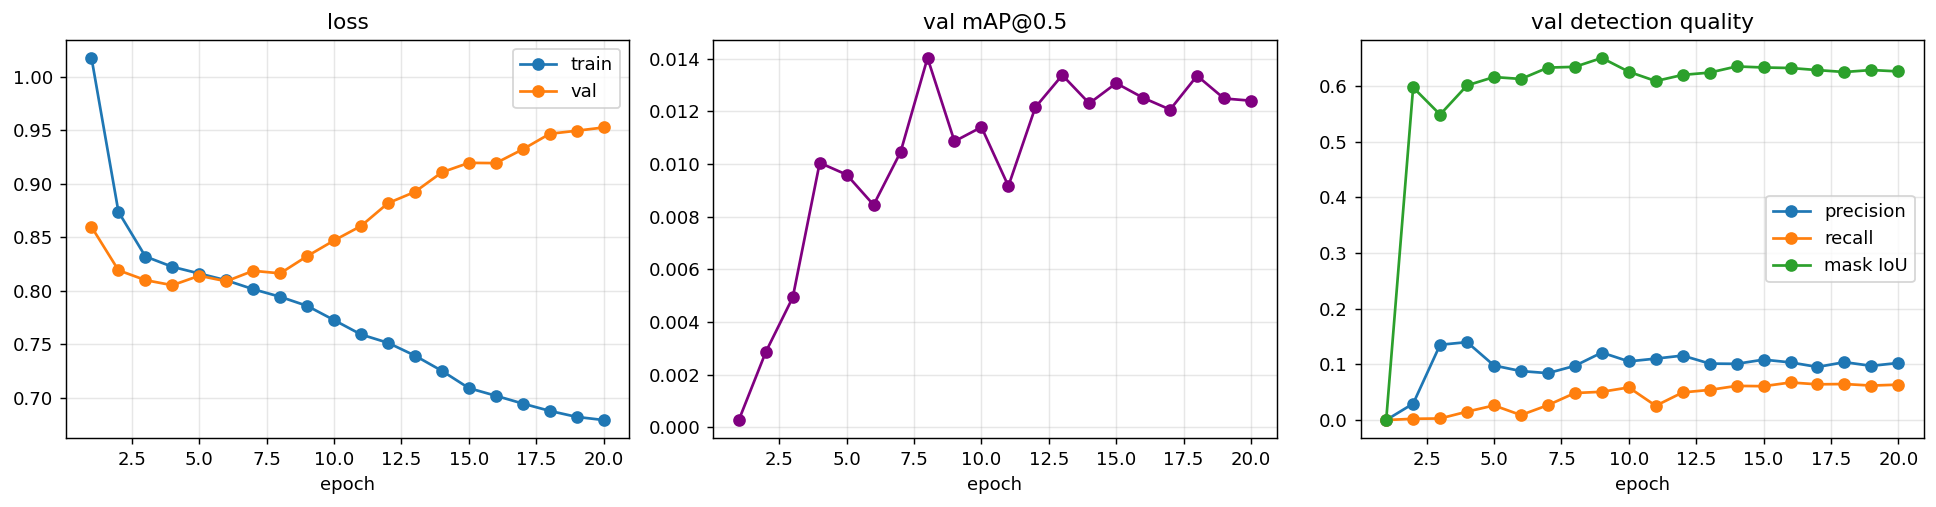
\includegraphics[width=\textwidth]{figures/training_curves.png}
\caption{Training history over $20$ epochs. \emph{Left:} train vs.\ validation
loss --- validation loss turns upward after $\sim\!4$ epochs, indicating
overfitting. \emph{Centre:} validation mAP@0.5, peaking near epoch~$8$.
\emph{Right:} detection quality --- mask IoU saturates early and high, while
precision and recall stay low. The decoupling of mask quality from detection
quality is the central result of this experiment.}
\label{fig:curves}
\end{figure*}

\begin{figure*}[p]
\centering
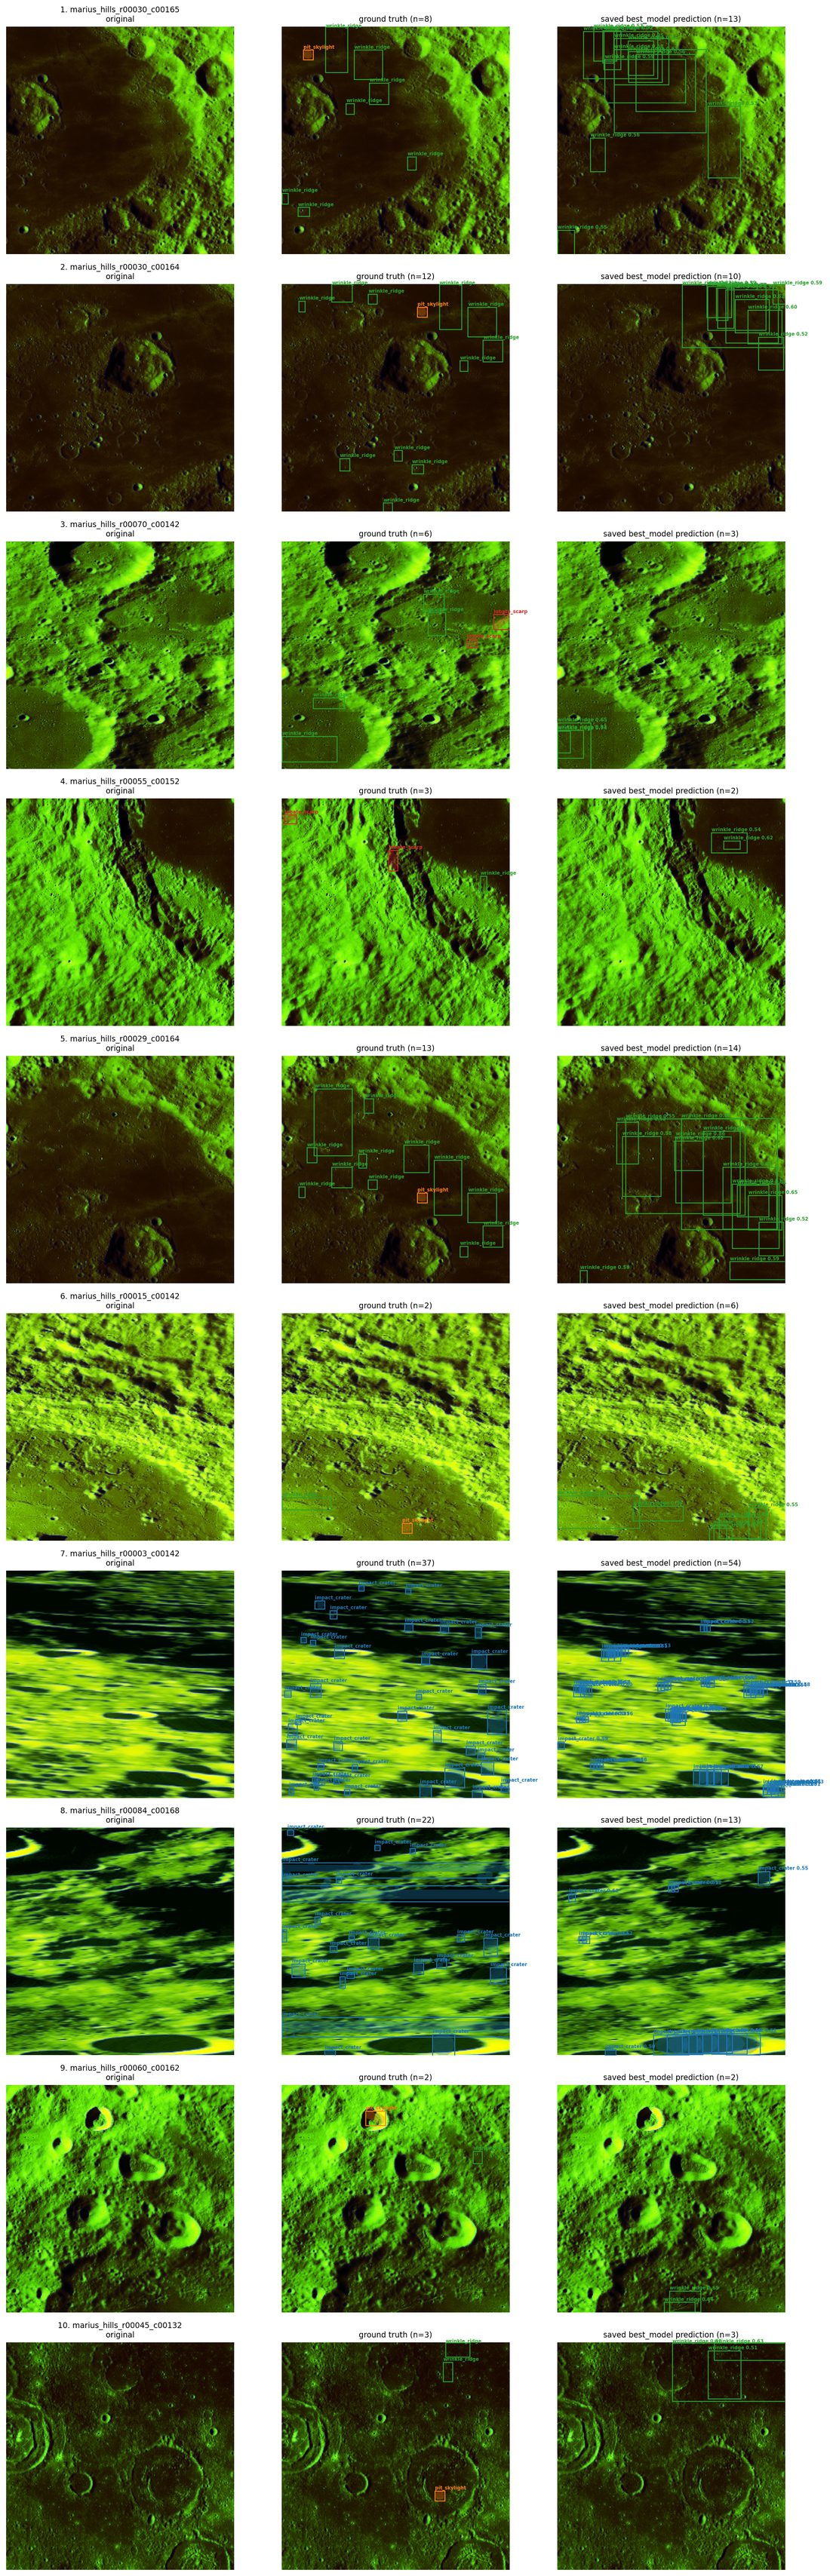
\includegraphics[height=0.92\textheight,keepaspectratio]{figures/prediction_samples.jpg}
\caption{Qualitative results on ten validation tiles from the Marius Hills region.
For each tile: original image (left), ground-truth instances (centre), and
model predictions with class and confidence (right). The network localises and
outlines the larger, higher-contrast craters and ridges reasonably well, but
misses faint or small features and is unreliable on the rare pit/skylight and
lobate-scarp classes.}
\label{fig:qual}
\end{figure*}

\section{SmallUNet: architecture details, losses, and full ablation results}
\label{app:unet}

\subsection{Architecture}

The spatial flow of the network with base width $w=32$ and $256\times 256$ input is:

\[
\begin{array}{c}
(3,\,256,256)
\xrightarrow{\text{inc}}   (32,\,256,256)\\[2pt]
\xrightarrow{\text{down}_1}(64,\,128,128)\\[2pt]
\xrightarrow{\text{down}_2}(128,\,64,64)\\[2pt]
\xrightarrow{\text{down}_3}(256,\,32,32)\\[4pt]
\xrightarrow{\text{up}_1}  (128,\,64,64)\\[2pt]
\xrightarrow{\text{up}_2}  (64,\,128,128)\\[2pt]
\xrightarrow{\text{up}_3}  (32,\,256,256)\\[2pt]
\xrightarrow{\text{out}}   (7,\,256,256)
\end{array}
\]

\noindent
Doubling the base width $w$ quadruples the parameter count; Table~\ref{tab:bw_params} summarises the three widths explored in Study~2.

\begin{table}[htbp]
\centering
\caption{Parameter counts for each base width.}
\label{tab:bw_params}
\begin{tabular}{lrr}
\toprule
Base width $w$ & Channel progression & Parameters \\
\midrule
16 & 16--32--64--128  &    505{,}095 \\
32 & 32--64--128--256 & 2{,}014{,}727 \\
64 & 64--128--256--512 & 8{,}047{,}623 \\
\bottomrule
\end{tabular}
\end{table}

\subsection{Loss definitions}

\paragraph{BCEDiceLoss.}
Binary cross-entropy summed with a soft Dice loss, averaged across classes:
\[
\mathcal{L}_{\text{BCEDice}} = \mathcal{L}_{\text{BCE}} + \mathcal{L}_{\text{Dice}},
\]
\[
\mathcal{L}_{\text{Dice}} = 1 - \frac{1}{C}\sum_{c=1}^{C} \frac{2\sum_i p_i^c\, y_i^c + \varepsilon}{\sum_i p_i^c + \sum_i y_i^c + \varepsilon}
\]
where $p_i^c$ is the predicted probability and $y_i^c$ the ground-truth label for pixel $i$ and class $c$, and $\varepsilon=10^{-6}$ ensures numerical stability.

\paragraph{FocalDiceLoss.}
Replaces the BCE term with the binary focal loss~\citep{lin2017focal} to down-weight easy negatives and focus training on hard positives:
\[
\mathcal{L}_{\text{focal}}(p,y) = -\alpha\,y\,(1-p)^\gamma \log p
                                   -(1-\alpha)(1-y)\,p^\gamma \log(1-p)
\]
with $\gamma=2$ and $\alpha=0.25$. The Dice term additionally uses per-class weights $\mathbf{w} = [1.0,\,4.0,\,5.0,\,5.0,\,5.0,\,5.0,\,5.0]$ to penalise misdetection of rare classes more heavily:
\[
\mathcal{L}_{\text{FocalDice}} = \mathcal{L}_{\text{focal}} + \sum_{c=1}^{C} w_c \,\mathcal{L}_{\text{Dice}}^c
\]

\subsection{Full ablation tables and validation curves}

Tables~\ref{tab:arch_comparison}--\ref{tab:aug_comparison} report the complete per-study results summarised in Sect.~\ref{sec:mr_augmentation}; Figs.~\ref{fig:arch_metrics}--\ref{fig:aug_metrics} show the corresponding per-class validation curves.

\begin{table}[htbp]
\centering
\caption{Architecture ablation on the full dataset (Tesla T4, 30 epochs). Metrics are macro-averaged across the seven classes; Ridge AP is the single-class AP of \texttt{wrinkle\_ridge}.}
\label{tab:arch_comparison}
\resizebox{\columnwidth}{!}{%
\begin{tabular}{lrrrrrrr}
\toprule
Config & Params & Epoch (s) & Final loss & Mean F1 & Mean IoU & Mean AP & Ridge AP \\
\midrule
BCEDice    & 1{,}927{,}207 & 208 & 0.876 & 0.1998 & 0.1666 & 0.1989 & 0.440 \\
FocalDice  & 1{,}927{,}207 & 214 & 3.893 & 0.1994 & 0.1632 & 0.1945 & 0.417 \\
+residual  & 2{,}014{,}727 & 257 & 3.873 & 0.2065 & 0.1675 & 0.1995 & 0.443 \\
+dropout   & 1{,}927{,}207 & 215 & 3.894 & 0.2018 & 0.1643 & 0.1938 & 0.405 \\
\textbf{+both} & \textbf{2{,}014{,}727} & 258 & \textbf{3.863} & \textbf{0.2076} & \textbf{0.1688} & \textbf{0.2004} & \textbf{0.453} \\
\bottomrule
\end{tabular}
}
\end{table}

\begin{table}[htbp]
\centering
\caption{Base-width sweep (FocalDice + residual + dropout=0.3, full T4 run, 30 epochs).}
\label{tab:bw_comparison}
\resizebox{\columnwidth}{!}{%
\begin{tabular}{lrrrrrr}
\toprule
Config & Params & Epoch (s) & Mean F1 & Mean IoU & Mean AP & Ridge AP \\
\midrule
small ($w=16$)   &    505{,}095 &  139 & 0.2031 & 0.1665 & 0.2003 & 0.451 \\
default ($w=32$) & 2{,}014{,}727 &  258 & 0.2093 & 0.1704 & 0.2010 & 0.456 \\
wide ($w=64$)    & 8{,}047{,}623 &  582 & \textbf{0.2153} & \textbf{0.1733} & \textbf{0.2016} & 0.445 \\
\bottomrule
\end{tabular}
}
\end{table}

\begin{table}[htbp]
\centering
\caption{Augmentation study on the random tile split (FocalDice + residual + dropout=0.3, $w=32$, full T4 run, 30 epochs). Crater AP is given for reference; Ridge AP highlights the most affected rare class.}
\label{tab:aug_comparison}
\resizebox{\columnwidth}{!}{%
\begin{tabular}{lrrrrrr}
\toprule
Config & Final loss & Mean F1 & Mean IoU & Mean AP & Crater AP & Ridge AP \\
\midrule
\textbf{no augmentation} & \textbf{3.698} & \textbf{0.2986} & \textbf{0.2289} & \textbf{0.2647} & \textbf{0.947} & \textbf{0.558} \\
+augmentation            &        3.863  &        0.2124  &        0.1724  &        0.2027  &        0.942  &        0.457  \\
\bottomrule
\end{tabular}
}
\end{table}

\begin{figure*}[htbp]
\centering
\begin{subfigure}[b]{0.32\textwidth}
    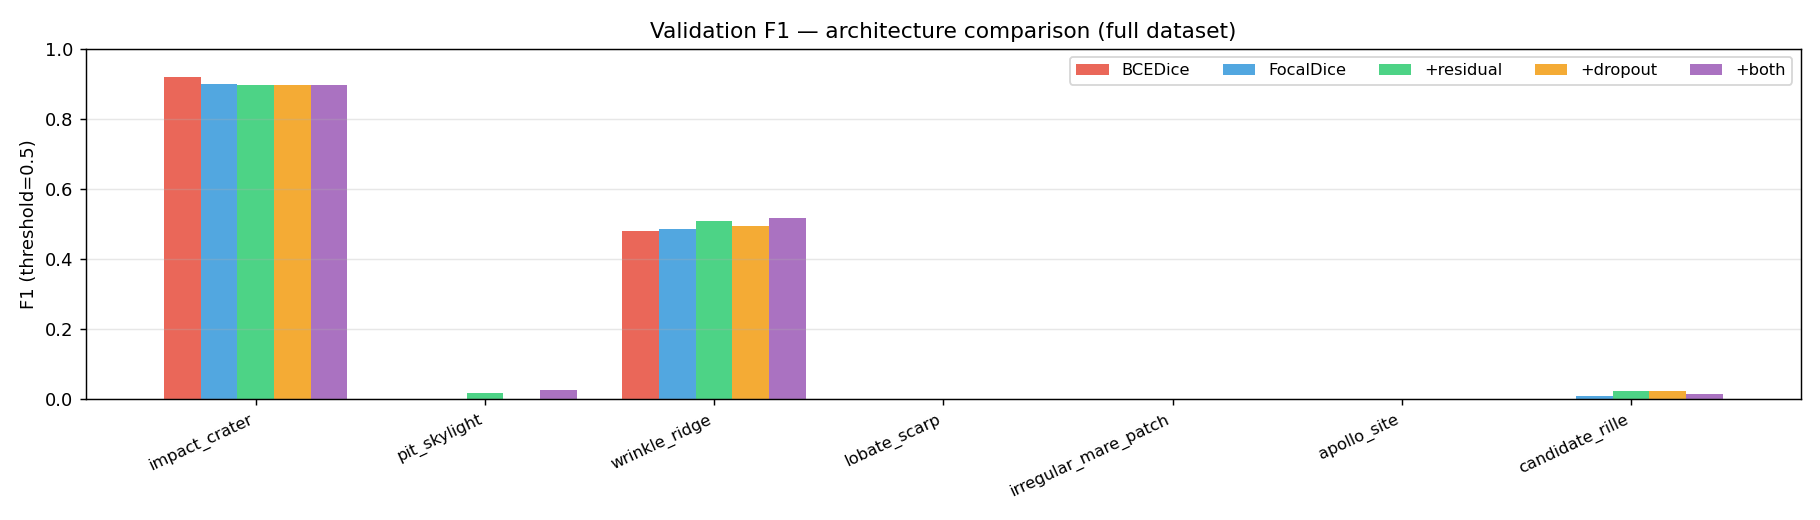
\includegraphics[width=\textwidth]{figures/MR/cloudveneto_arch_val_f1.png}
    \caption{Validation F1}
\end{subfigure}
\hfill
\begin{subfigure}[b]{0.32\textwidth}
    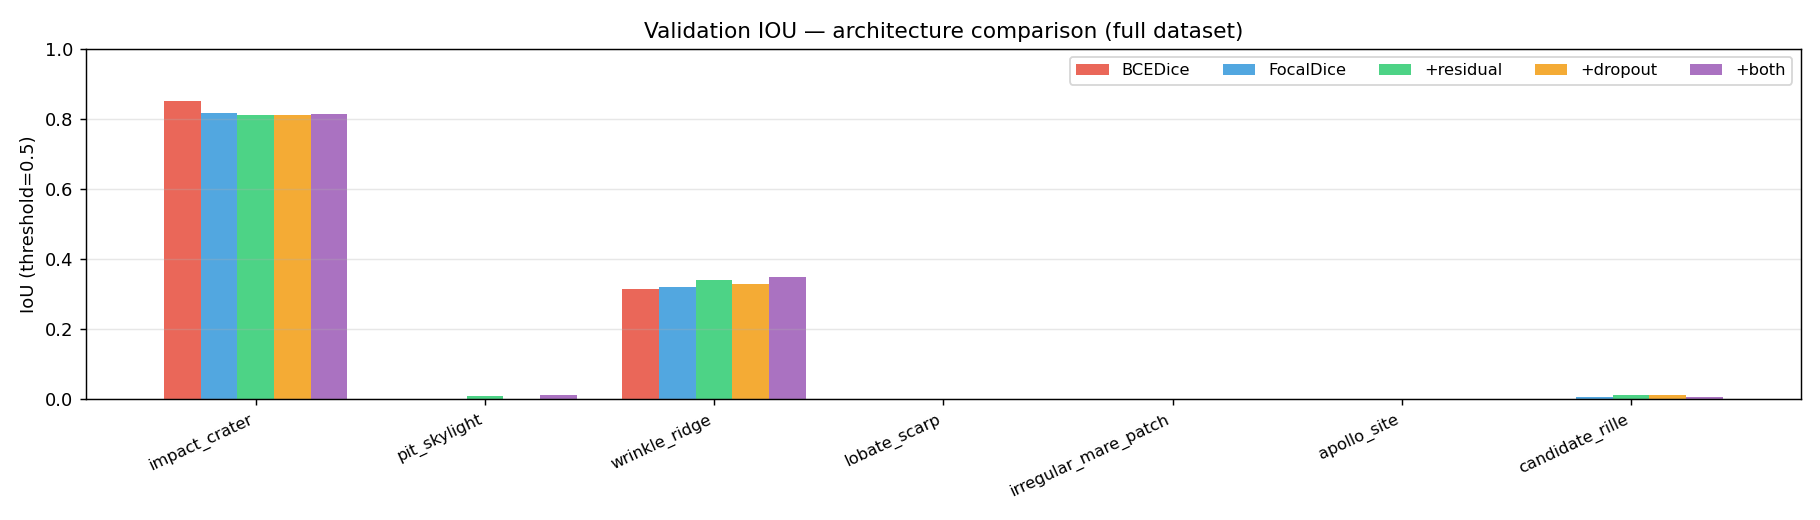
\includegraphics[width=\textwidth]{figures/MR/cloudveneto_arch_val_iou.png}
    \caption{Validation IoU}
\end{subfigure}
\hfill
\begin{subfigure}[b]{0.32\textwidth}
    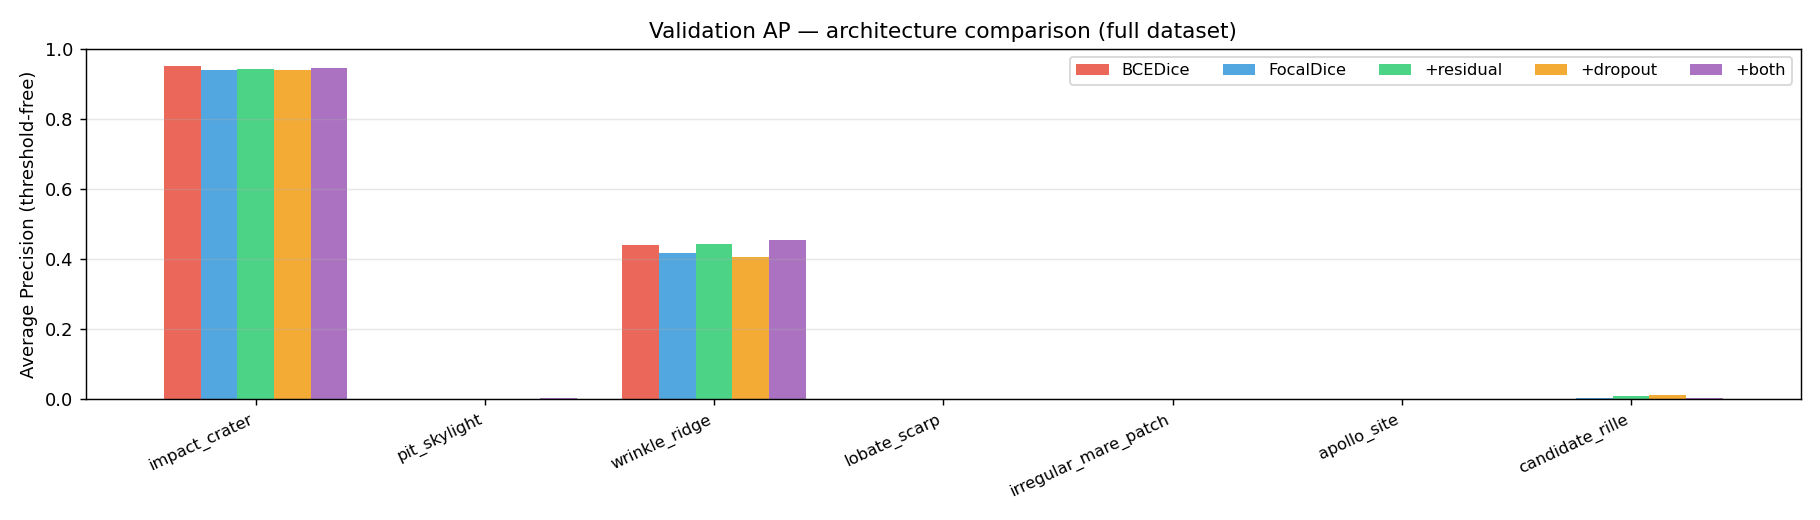
\includegraphics[width=\textwidth]{figures/MR/cloudveneto_arch_val_ap.png}
    \caption{Validation AP}
\end{subfigure}
\caption{Per-class validation metrics across training epochs for the five architecture configurations (full T4 run, 30 epochs). \textbf{+both} (residual + dropout + FocalDice) achieves the highest aggregate performance on all three metrics.}
\label{fig:arch_metrics}
\end{figure*}

\begin{figure*}[htbp]
\centering
\begin{subfigure}[b]{0.32\textwidth}
    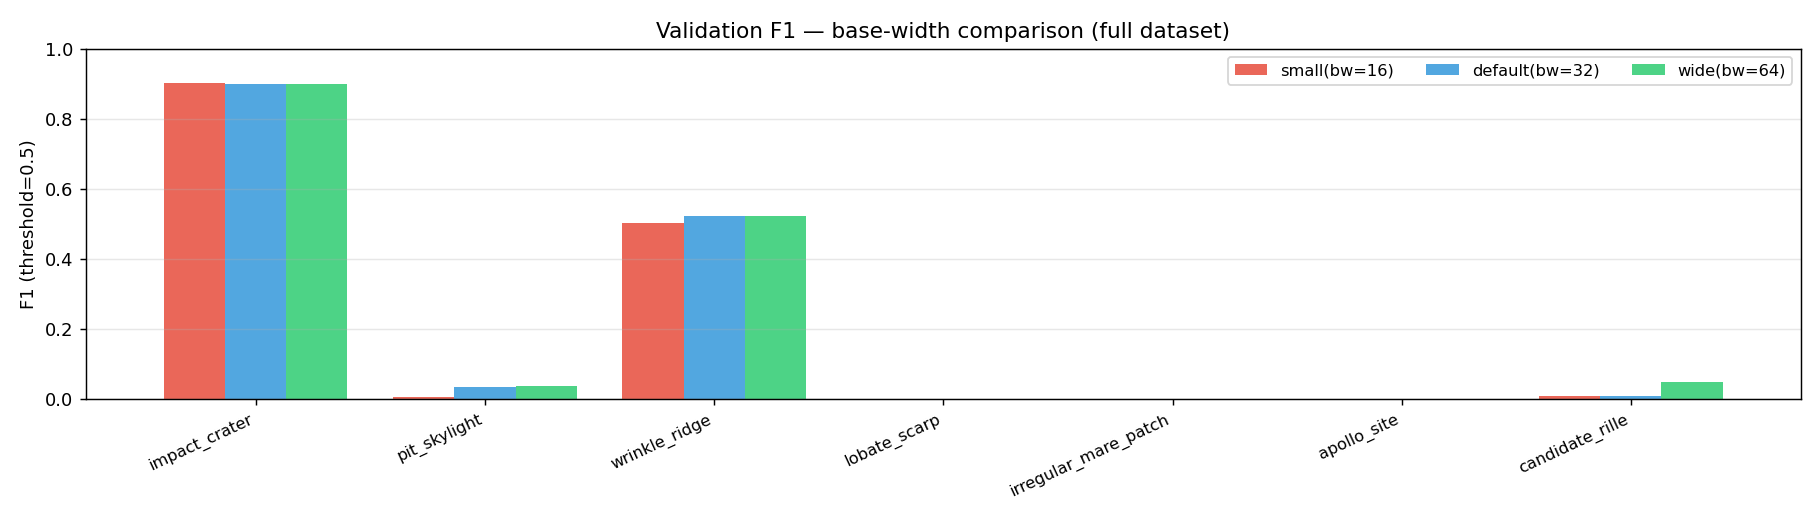
\includegraphics[width=\textwidth]{figures/MR/cloudveneto_bw_val_f1.png}
    \caption{Validation F1}
\end{subfigure}
\hfill
\begin{subfigure}[b]{0.32\textwidth}
    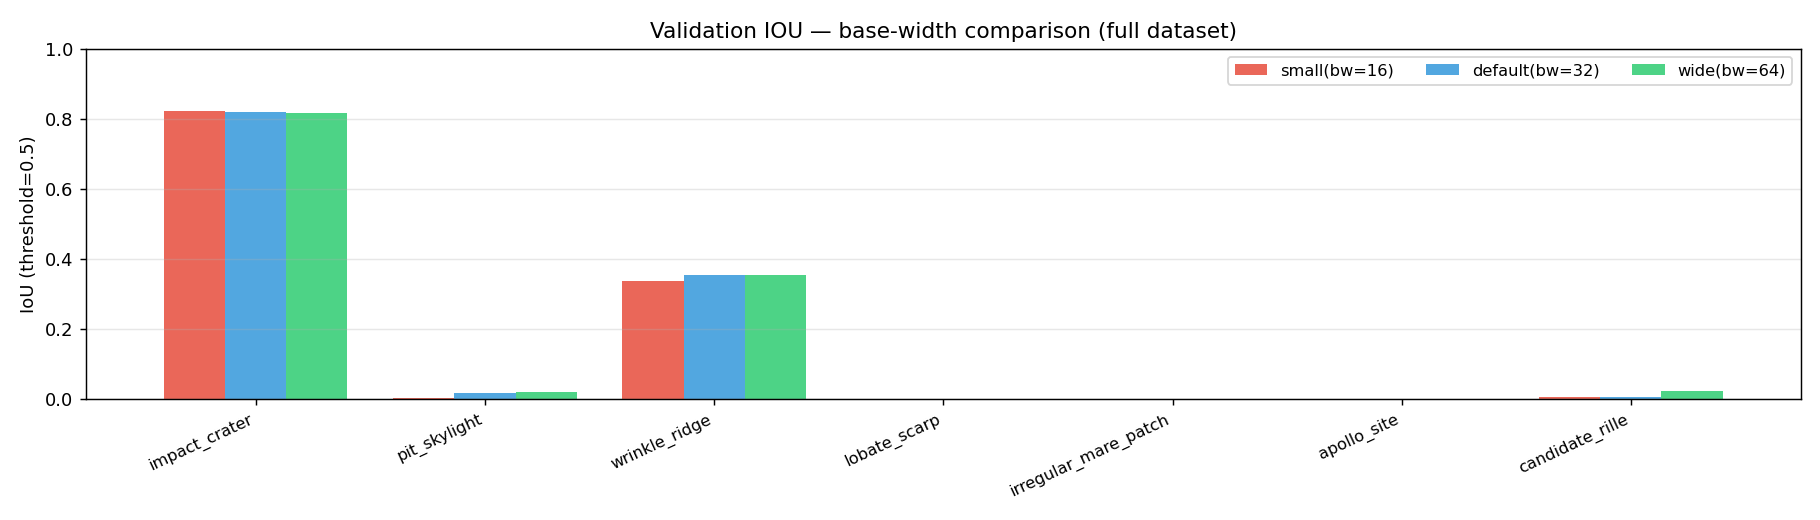
\includegraphics[width=\textwidth]{figures/MR/cloudveneto_bw_val_iou.png}
    \caption{Validation IoU}
\end{subfigure}
\hfill
\begin{subfigure}[b]{0.32\textwidth}
    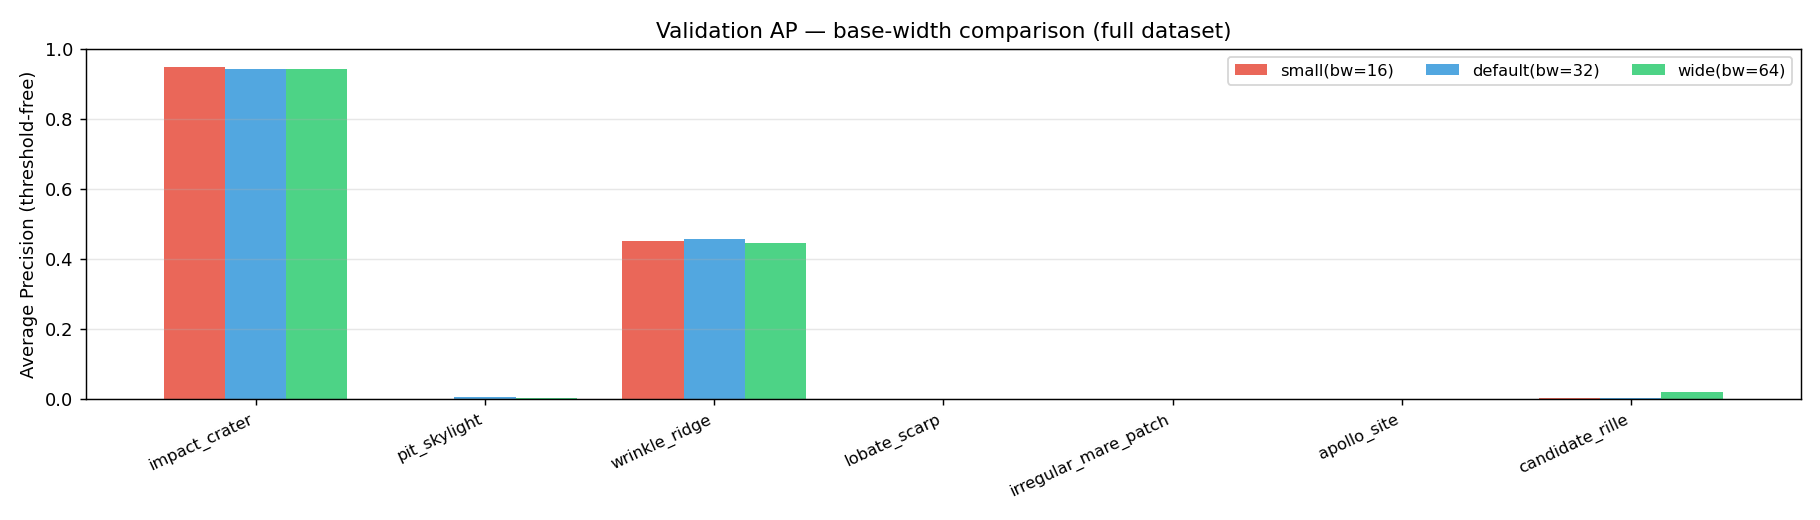
\includegraphics[width=\textwidth]{figures/MR/cloudveneto_bw_val_ap.png}
    \caption{Validation AP}
\end{subfigure}
\caption{Validation metrics for three network widths (full T4 run, 30 epochs). Wider networks achieve marginally higher scores but exhibit severely diminishing returns in parameters and training time.}
\label{fig:bw_metrics}
\end{figure*}

\begin{figure*}[htbp]
\centering
\begin{subfigure}[b]{0.32\textwidth}
    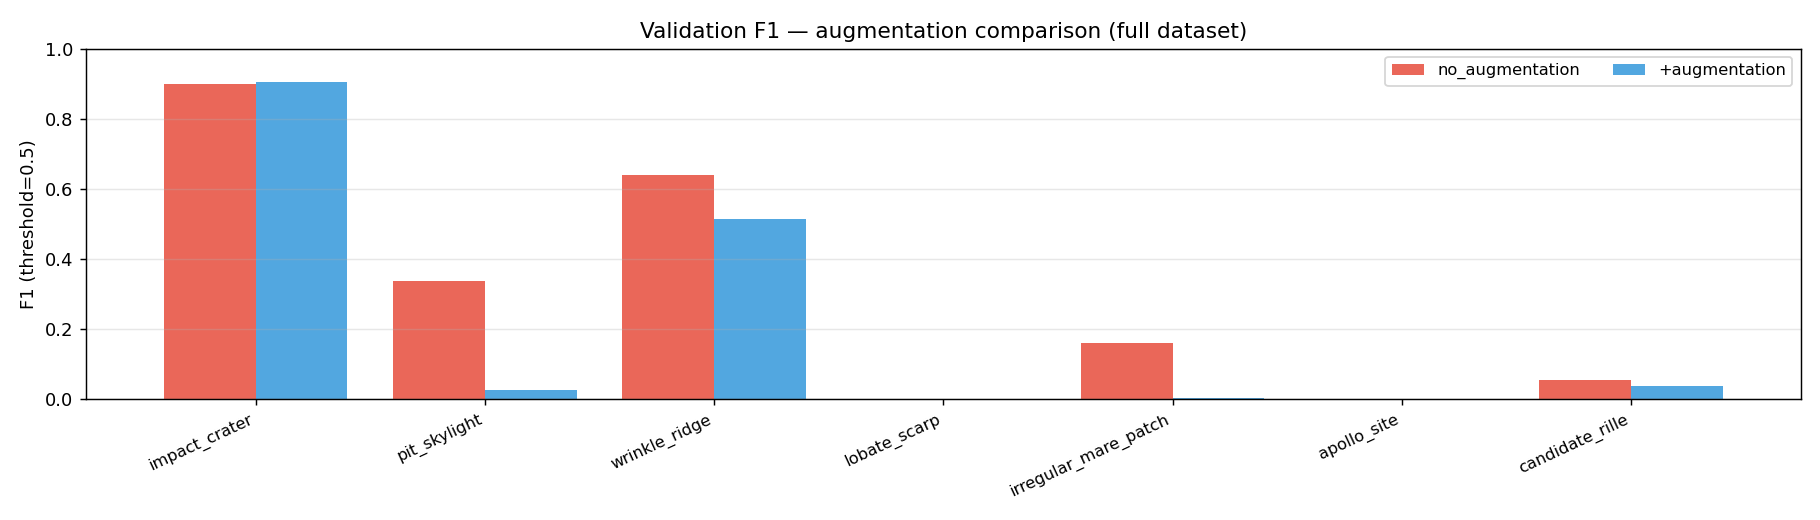
\includegraphics[width=\textwidth]{figures/MR/cloudveneto_aug_val_f1.png}
    \caption{Validation F1}
\end{subfigure}
\hfill
\begin{subfigure}[b]{0.32\textwidth}
    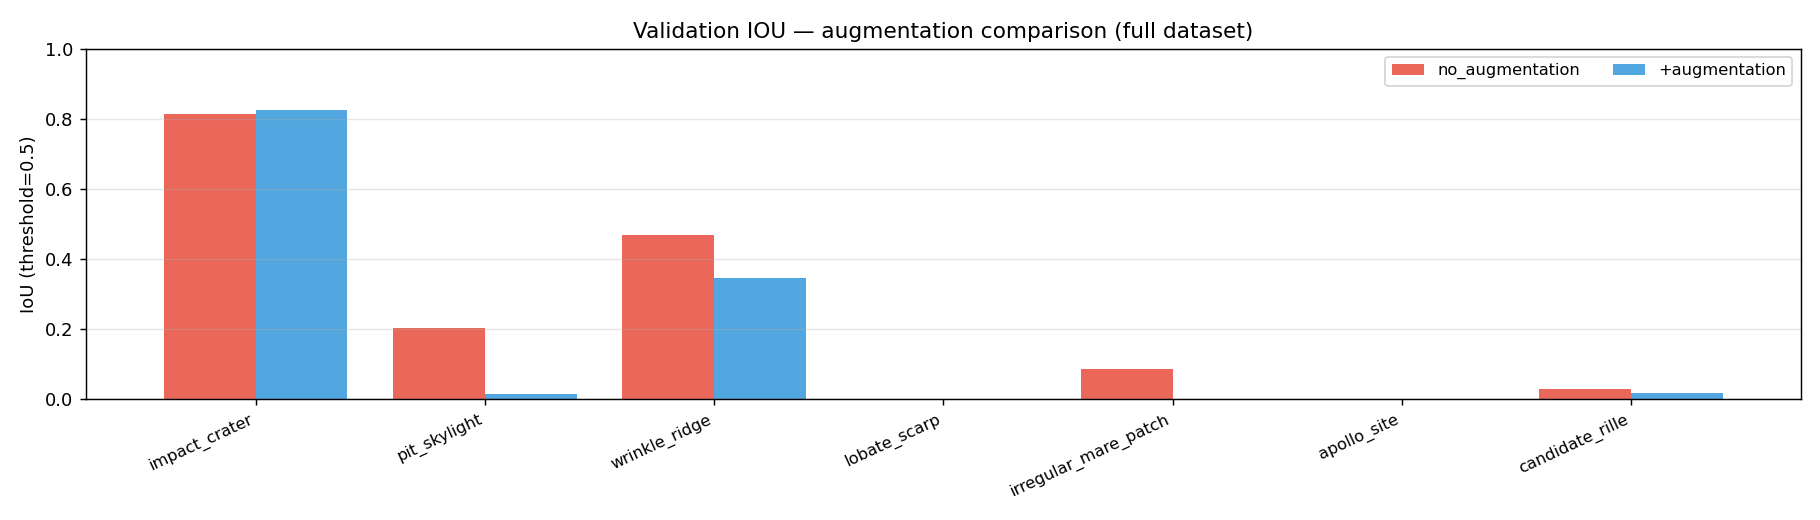
\includegraphics[width=\textwidth]{figures/MR/cloudveneto_aug_val_iou.png}
    \caption{Validation IoU}
\end{subfigure}
\hfill
\begin{subfigure}[b]{0.32\textwidth}
    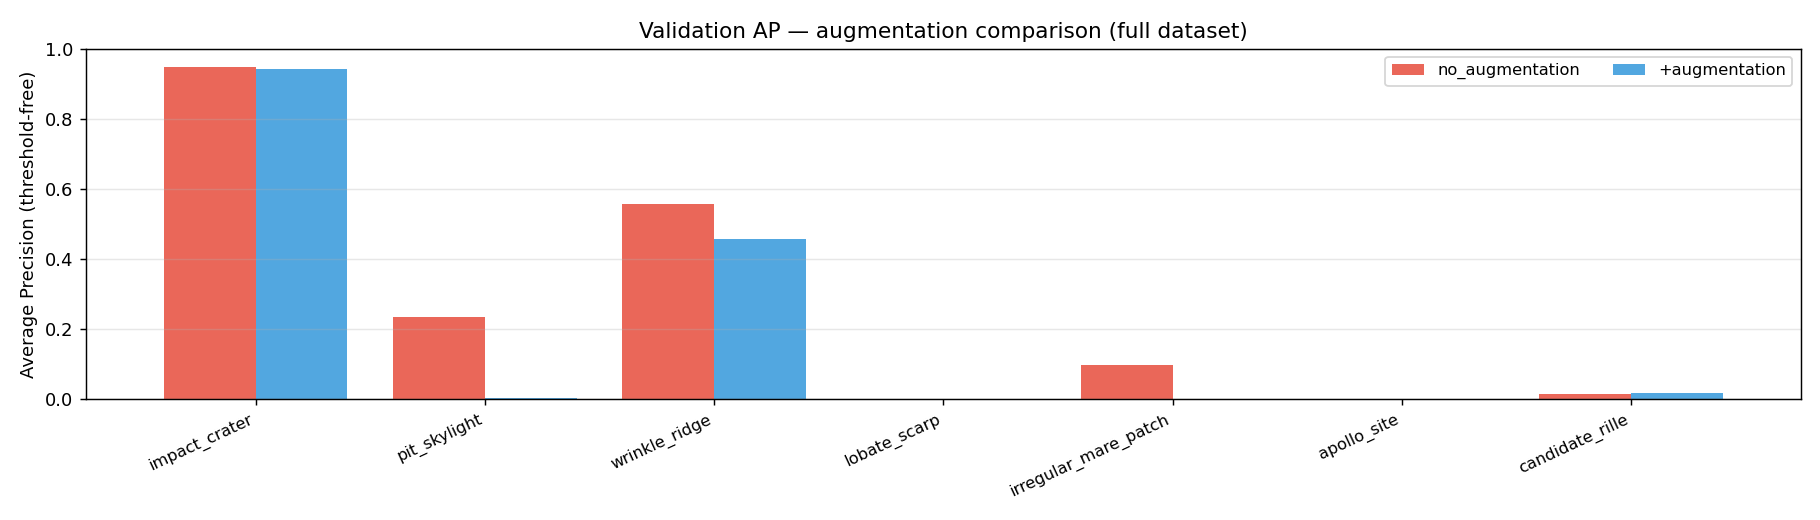
\includegraphics[width=\textwidth]{figures/MR/cloudveneto_aug_val_ap.png}
    \caption{Validation AP}
\end{subfigure}
\caption{Validation metrics with and without geometric augmentation (random tile split, full T4 run, 30 epochs). No augmentation outperforms the augmented training on all metrics.}
\label{fig:aug_metrics}
\end{figure*}

\subsection{Qualitative evaluation}

\begin{figure}[htbp!]
\centering
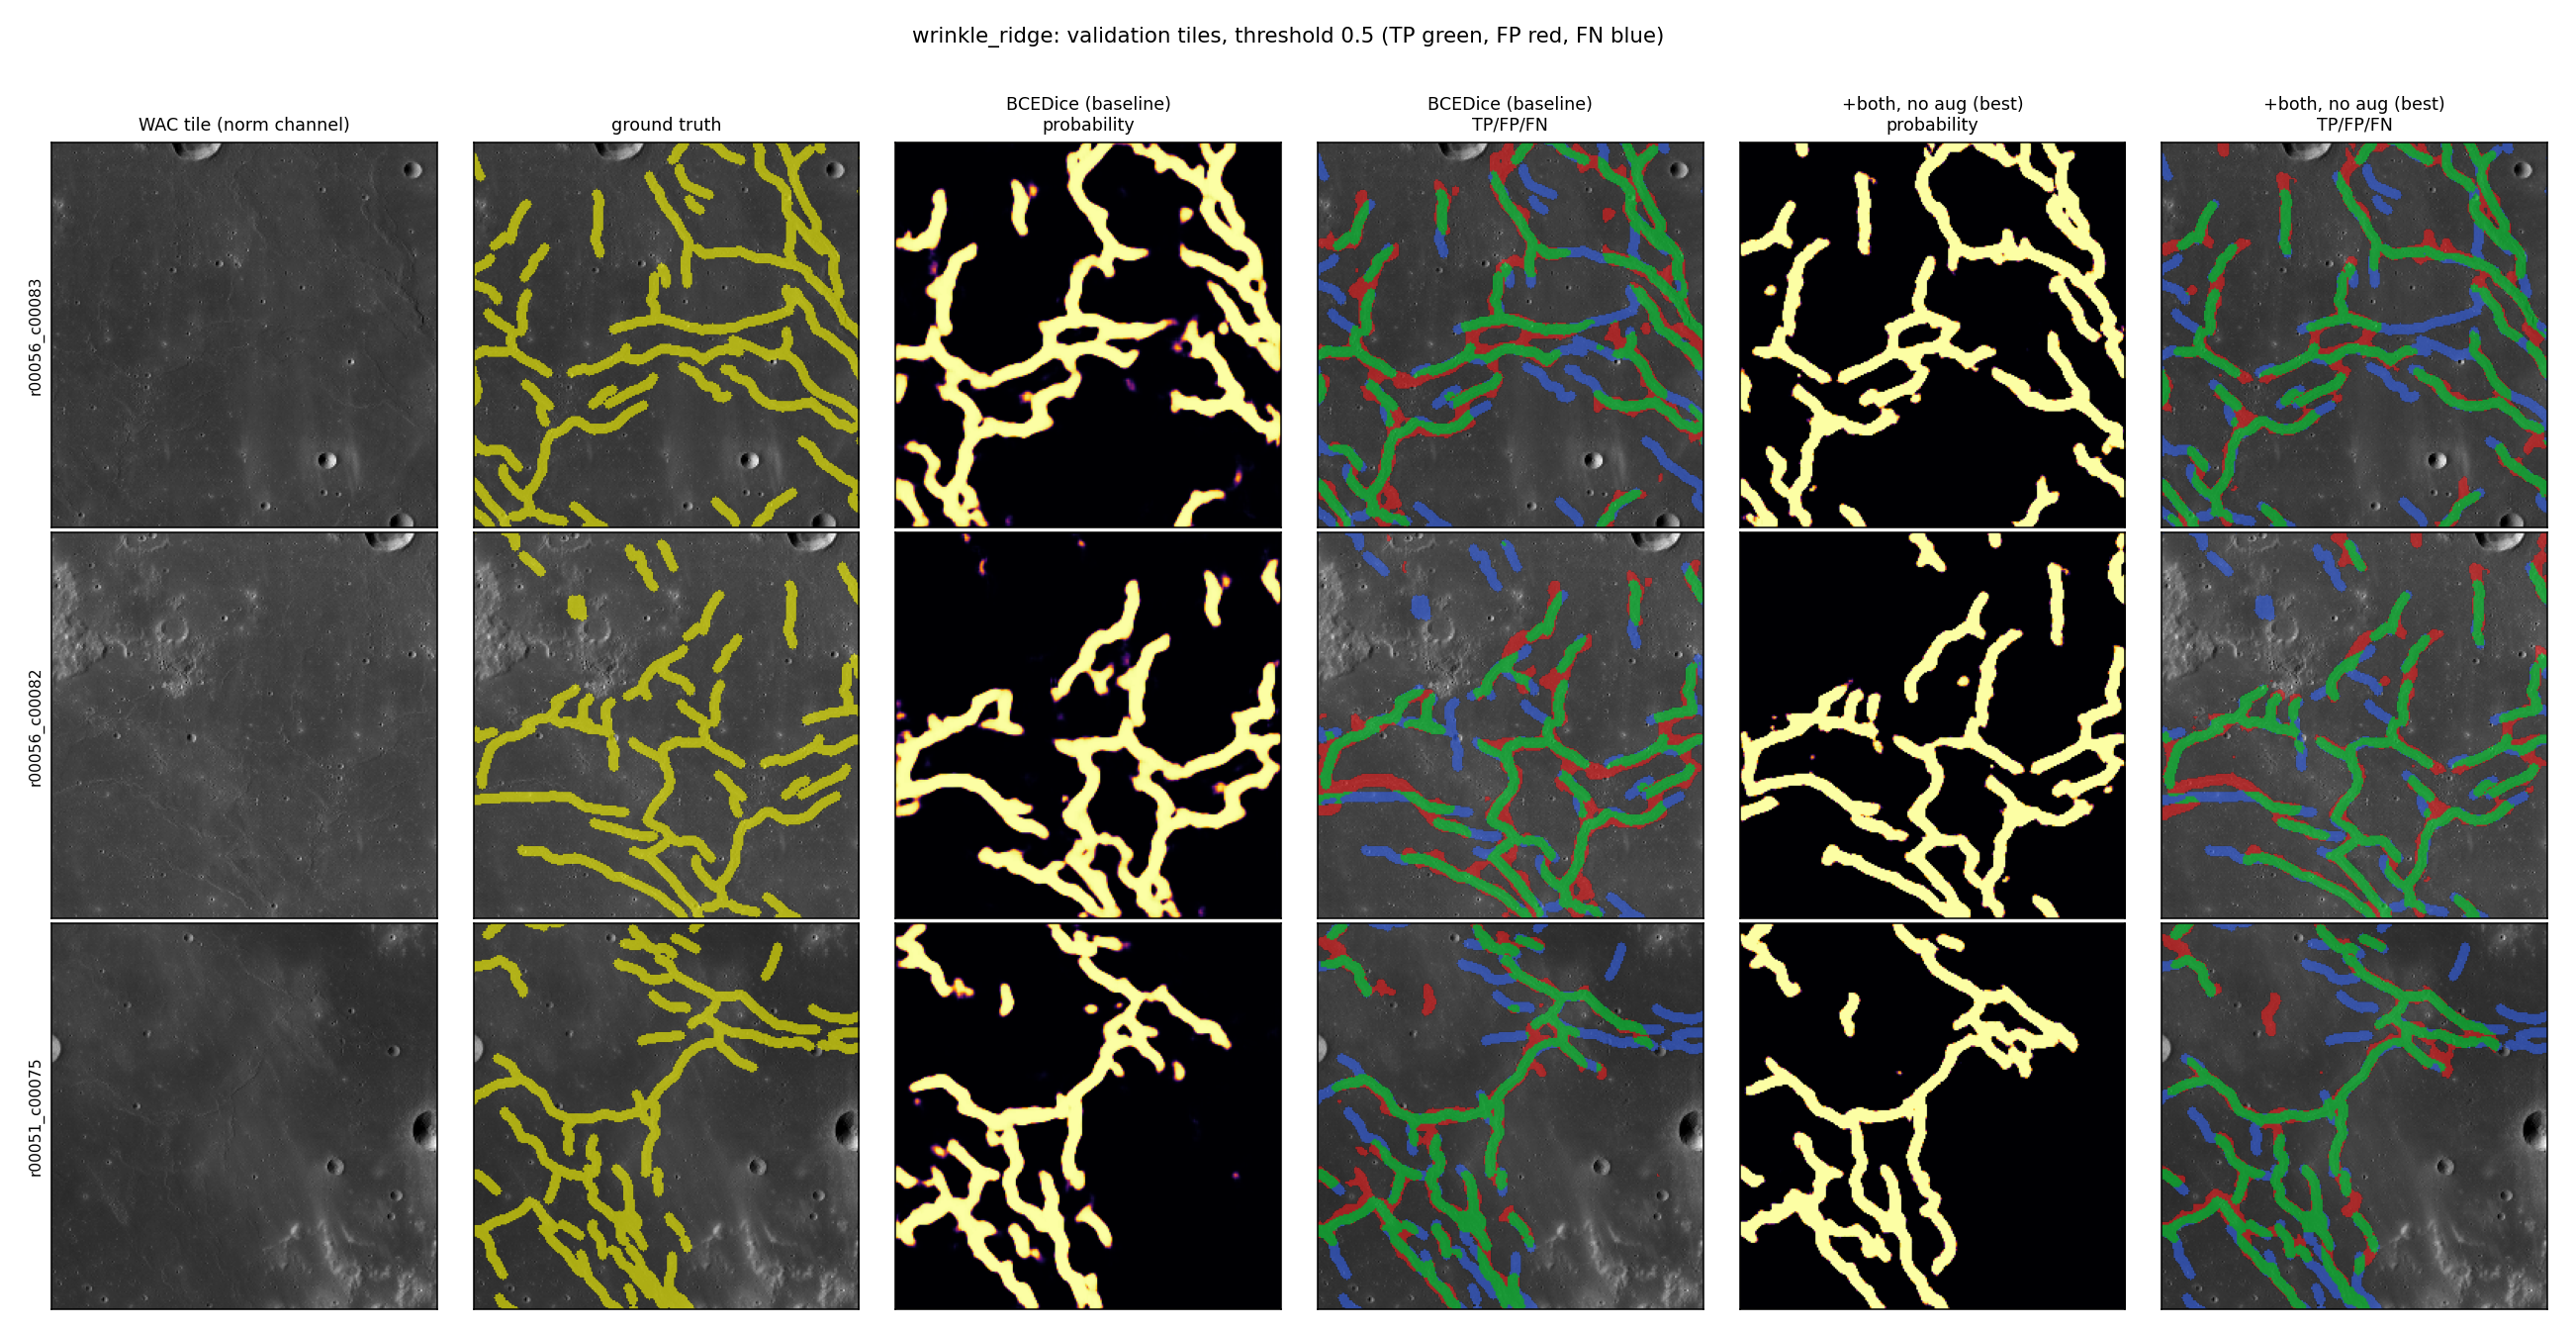
\includegraphics[width=0.85\columnwidth,keepaspectratio]{figures/MR/qualitative_wrinkle_ridge.png}
\caption{Wrinkle-ridge qualitative comparison on three validation tiles (TP green, FP red, FN blue). Both models recover the topology of the ridge network; the definitive model (+both, no augmentation) produces visibly more complete coverage and fewer false positives than the BCEDice baseline. Errors concentrate on thin, low-contrast ridge segments, consistent with the localisation difficulty of linear features.}
\label{fig:qualitative_ridge}
\end{figure}

\begin{figure}[htbp!]
\centering
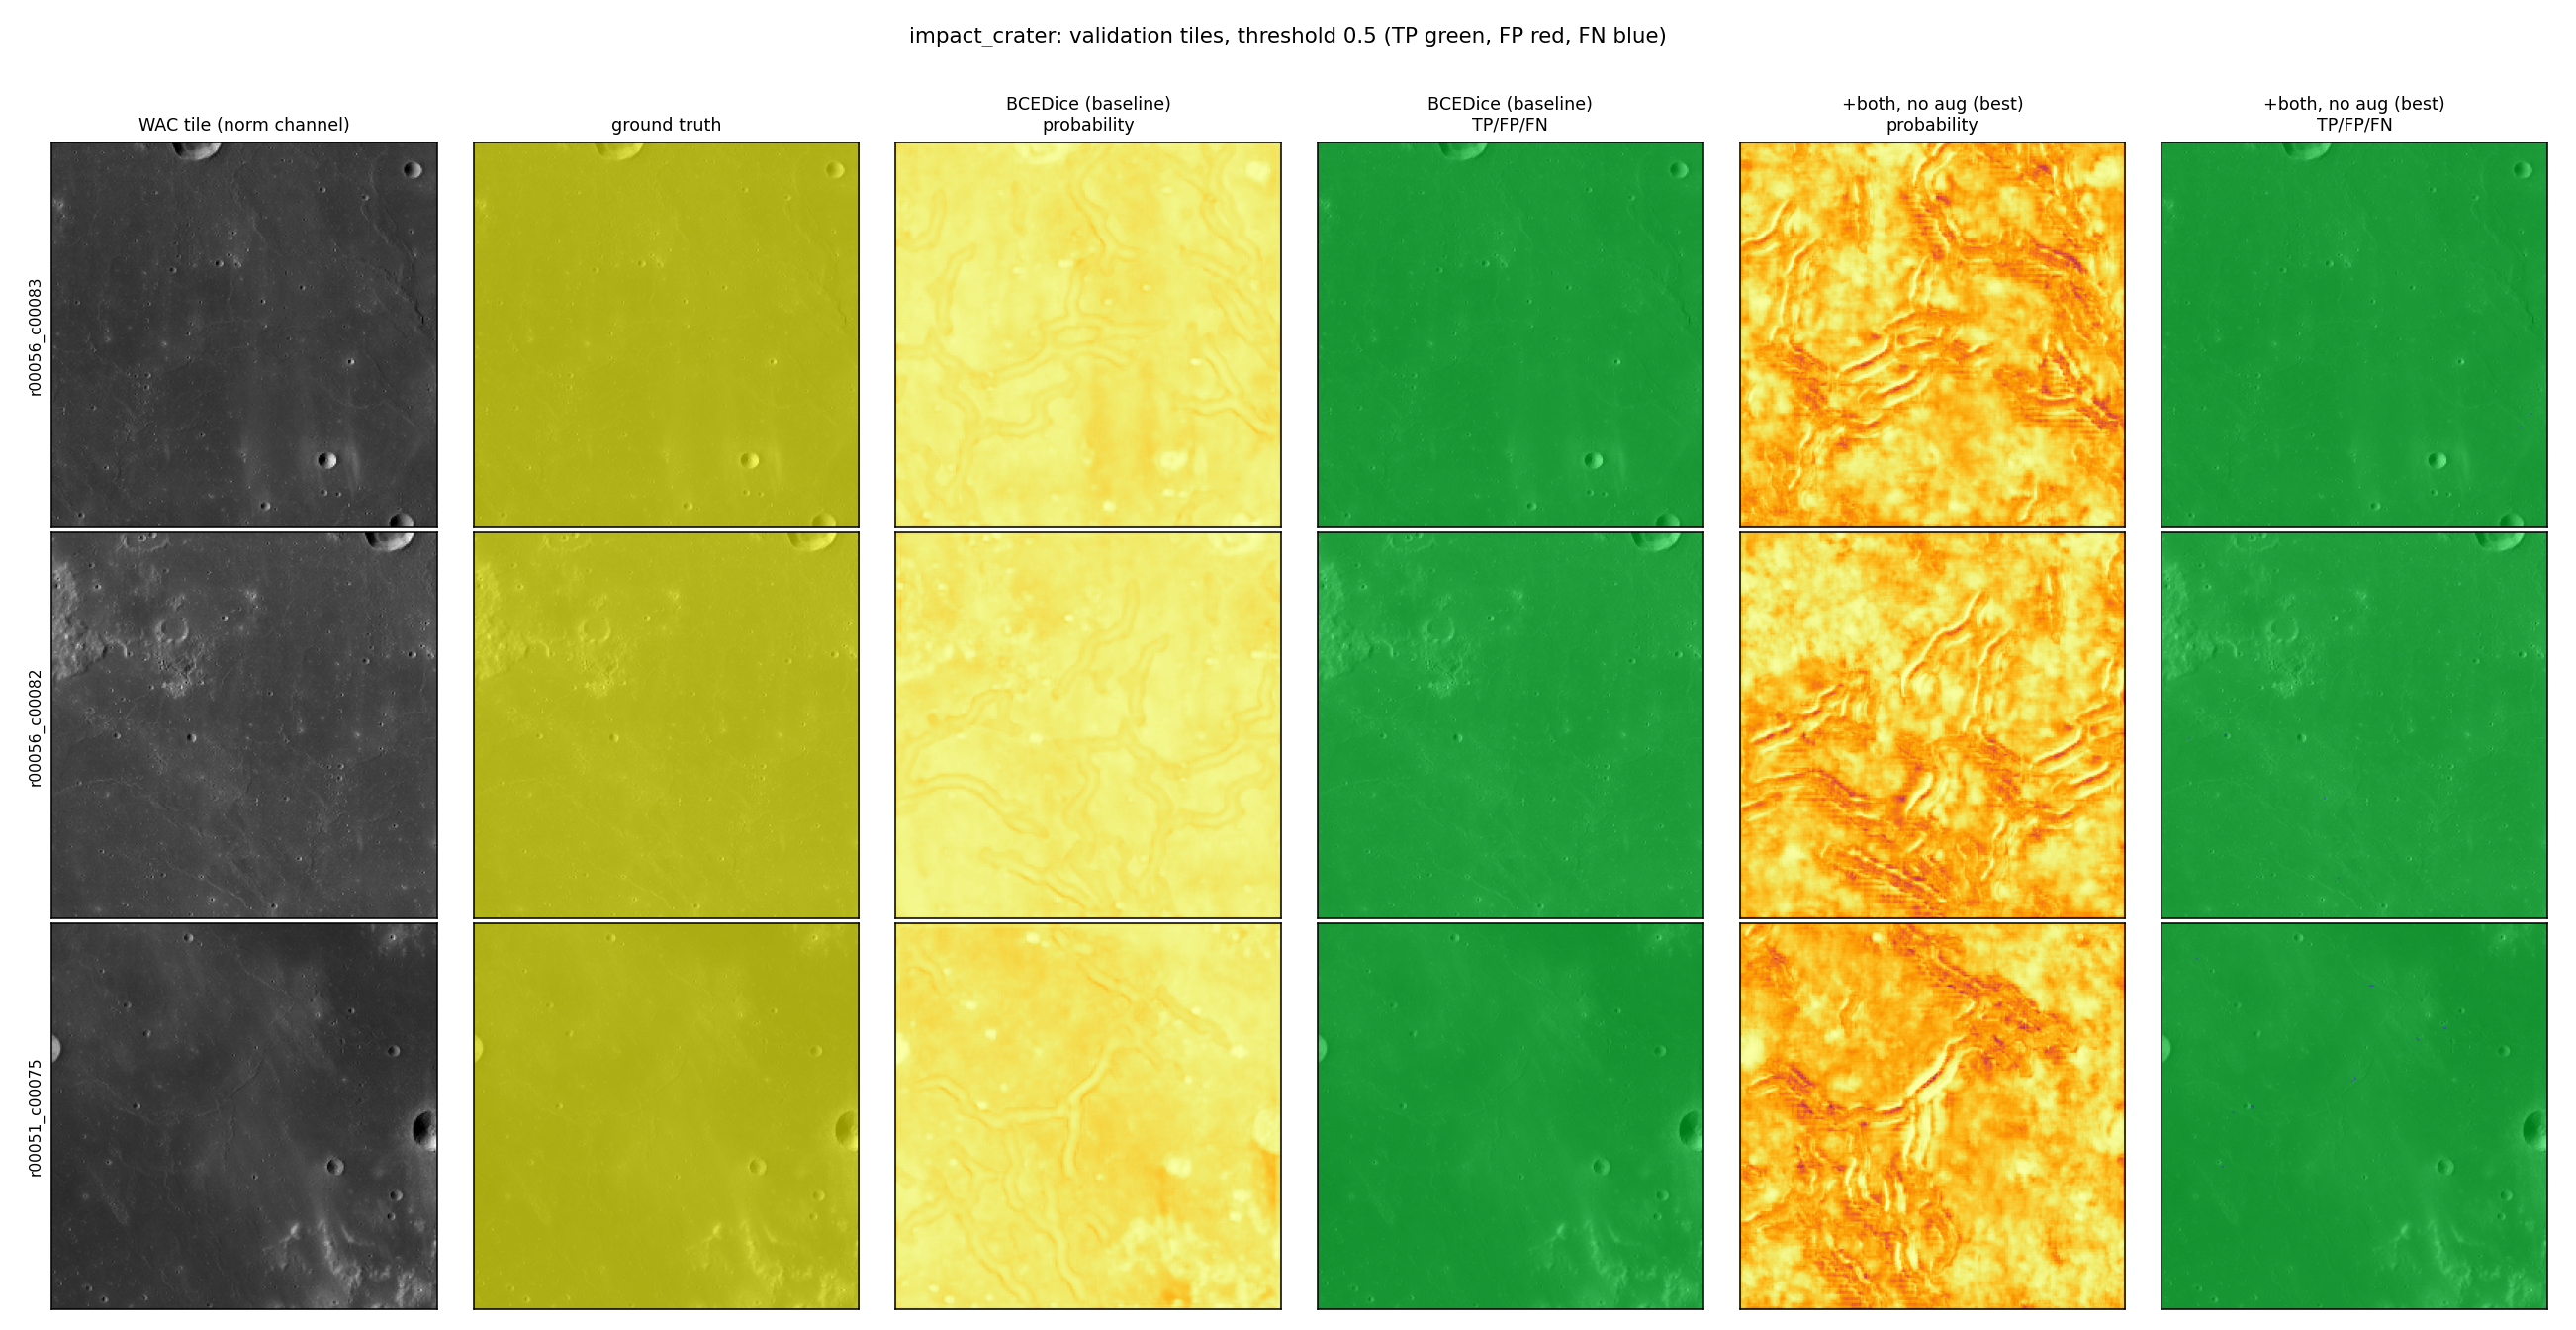
\includegraphics[width=0.85\columnwidth,keepaspectratio]{figures/MR/qualitative_impact_crater.png}
\caption{Impact-crater qualitative comparison on the same tiles. The ground truth covers the \emph{entire} tile (cf.\ the 82\% prevalence and 50.7\% fully-covered tiles of Table~\ref{tab:prevalence}), so a prediction of ``everywhere'' is trivially correct: this figure is direct visual evidence that the crater channel behaves as a near-coverage layer and that crater AP must be read against its 0.821 chance baseline.}
\label{fig:qualitative_crater}
\end{figure}

\section{YOLOv8: label statistics and training diagnostics}
\label{app:yolo}

Tables~\ref{tab:class_dist} and~\ref{tab:class_dist_reduced} report the box-level class distributions of the two training datasets of Sect.~\ref{sec:yolo}; Figs.~\ref{fig:class_dist}--\ref{fig:metrics_comparison} collect the label statistics and training diagnostics.

\begin{table}[htbp]
\centering
\caption{Per-class instance distribution in the full lunar surface feature dataset.}
\label{tab:class_dist}
\resizebox{\columnwidth}{!}{%
\begin{tabular}{llrr}
\hline
\textbf{Class ID} & \textbf{Class Label} & \textbf{Instances} & \textbf{Proportion (\%)} \\
\hline
class0 & Impact Crater         & 382,122 & 95.51 \\
class2 & Wrinkle Ridge         &  16,133 &  4.03 \\
class3 & Lobate Scarp          &     674 &  0.17 \\
class1 & Pit Skylight          &     328 &  0.08 \\
class4 & Irregular Mare Patch  &     191 &  0.05 \\
class5 & Apollo Site           &     161 &  0.04 \\
class6 & Candidate Rille       &      82 &  0.02 \\
\hline
\textbf{Total} & & \textbf{399,691} & \textbf{100.00} \\
\hline
\end{tabular}
}
\end{table}

\begin{table}[htbp]
\centering
\caption{Per-class instance distribution of the reduced dataset after excluding the impact crater class.}
\label{tab:class_dist_reduced}
\resizebox{\columnwidth}{!}{%
\begin{tabular}{llrr}
\hline
\textbf{Class ID} & \textbf{Class Label} & \textbf{Instances} & \textbf{Proportion (\%)} \\
\hline
class1 & Wrinkle Ridge        & 16,115 & 92.59 \\
class2 & Lobate Scarp         &    664 &  3.81 \\
class0 & Pit Skylight         &    311 &  1.79 \\
class4 & Apollo Site          &    156 &  0.90 \\
class3 & Irregular Mare Patch &    148 &  0.85 \\
class5 & Candidate Rille      &     92 &  0.53 \\
\hline
\textbf{Total} & & \textbf{17,486} & \textbf{100.00} \\
\hline
\end{tabular}
}
\end{table}

\begin{figure}[htbp!]
    \centering
    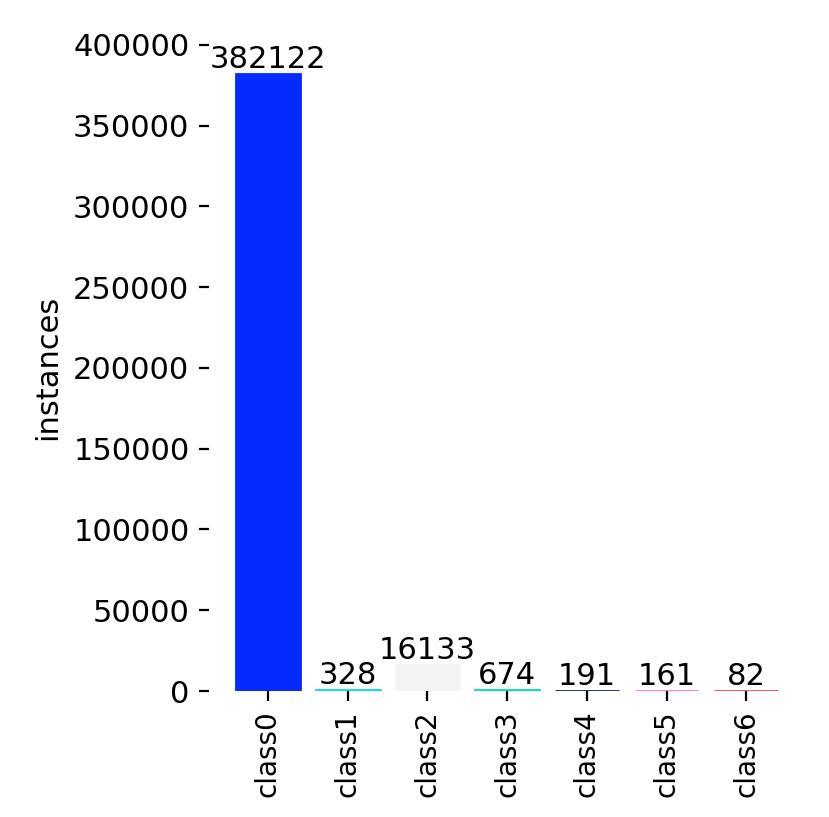
\includegraphics[width=0.85\linewidth]{./imageswithzero/labels_copy.jpg}
    \caption{Class instance distribution of the full dataset across
    seven categories. The impact crater class (class0) dominates with 382,122 instances,
    representing 95.51\% of all annotations.}
    \label{fig:class_dist}
\end{figure}

\begin{figure}[htbp!]
    \centering
    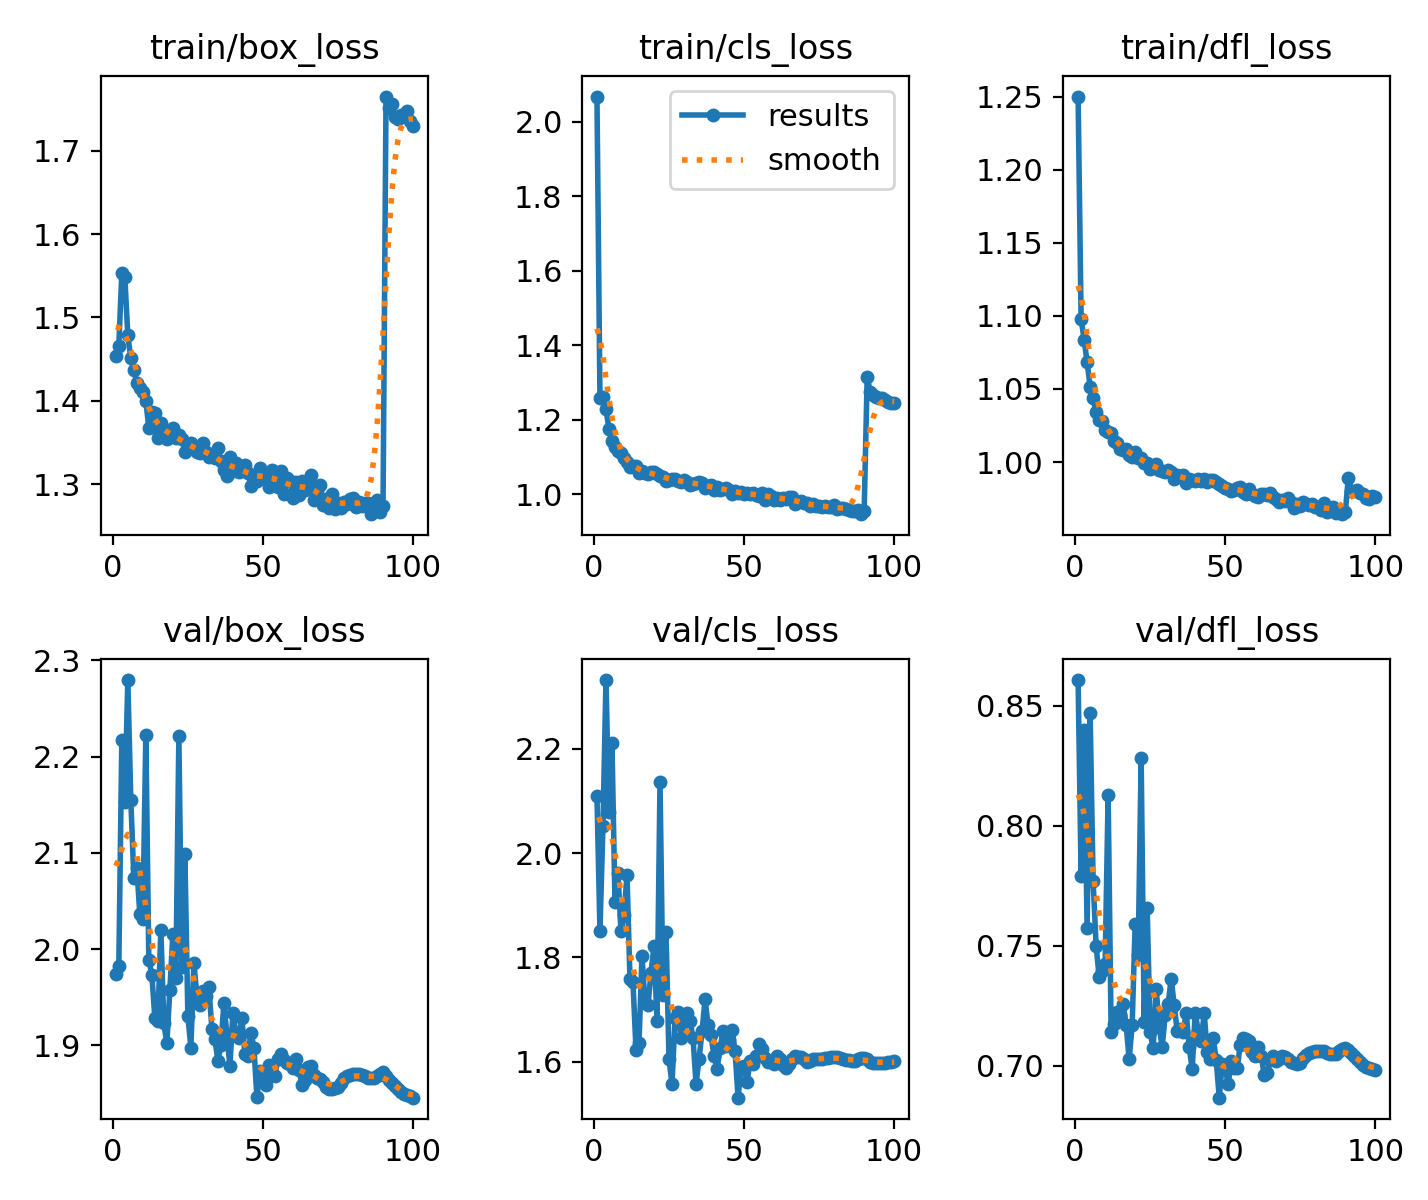
\includegraphics[width=0.95\linewidth]{./imageswithzero/loss.png}
    \caption{Training and validation loss curves over 100 epochs for the YOLOv8n
    model trained on the full seven-class dataset, including bounding box loss (box\_loss),
    classification loss (cls\_loss), and distribution focal loss (dfl\_loss).}
    \label{fig:loss_curves}
\end{figure}

\begin{figure}[htbp!]
    \centering
    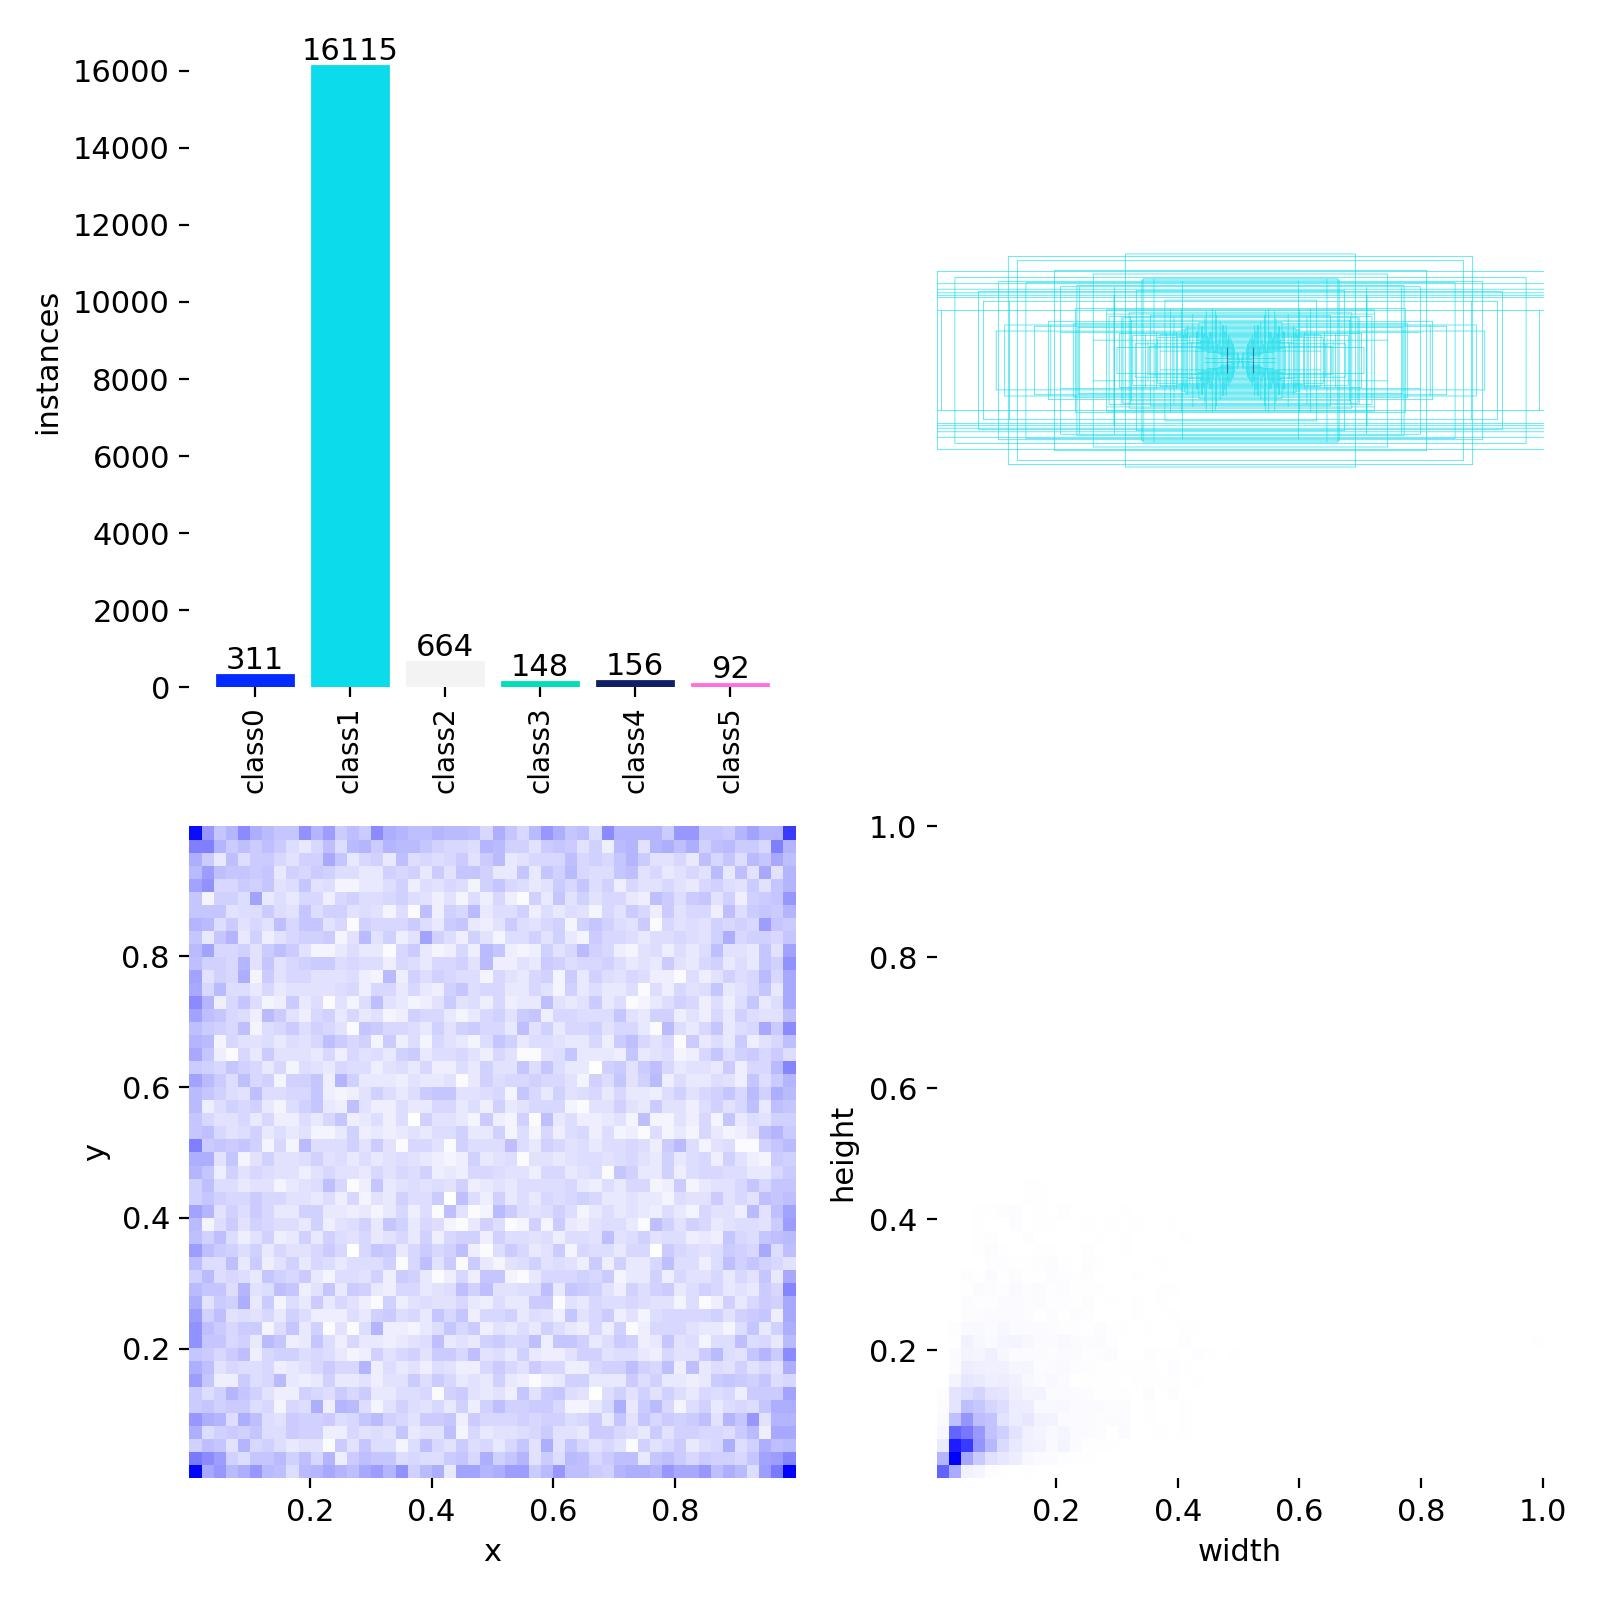
\includegraphics[width=0.85\linewidth]{imageswithoutzero/labels(1).jpg}
    \caption{Class instance distribution and spatial statistics of the reduced
    dataset after removing the impact crater class. The spatial heatmap shows a
    more uniform distribution of object centers across the image plane, while
    bounding boxes remain concentrated at small width-height values ($<$0.2),
    confirming the small-scale nature of the detected features.}
    \label{fig:labels_reduced}
\end{figure}

\begin{figure}[htbp!]
    \centering
    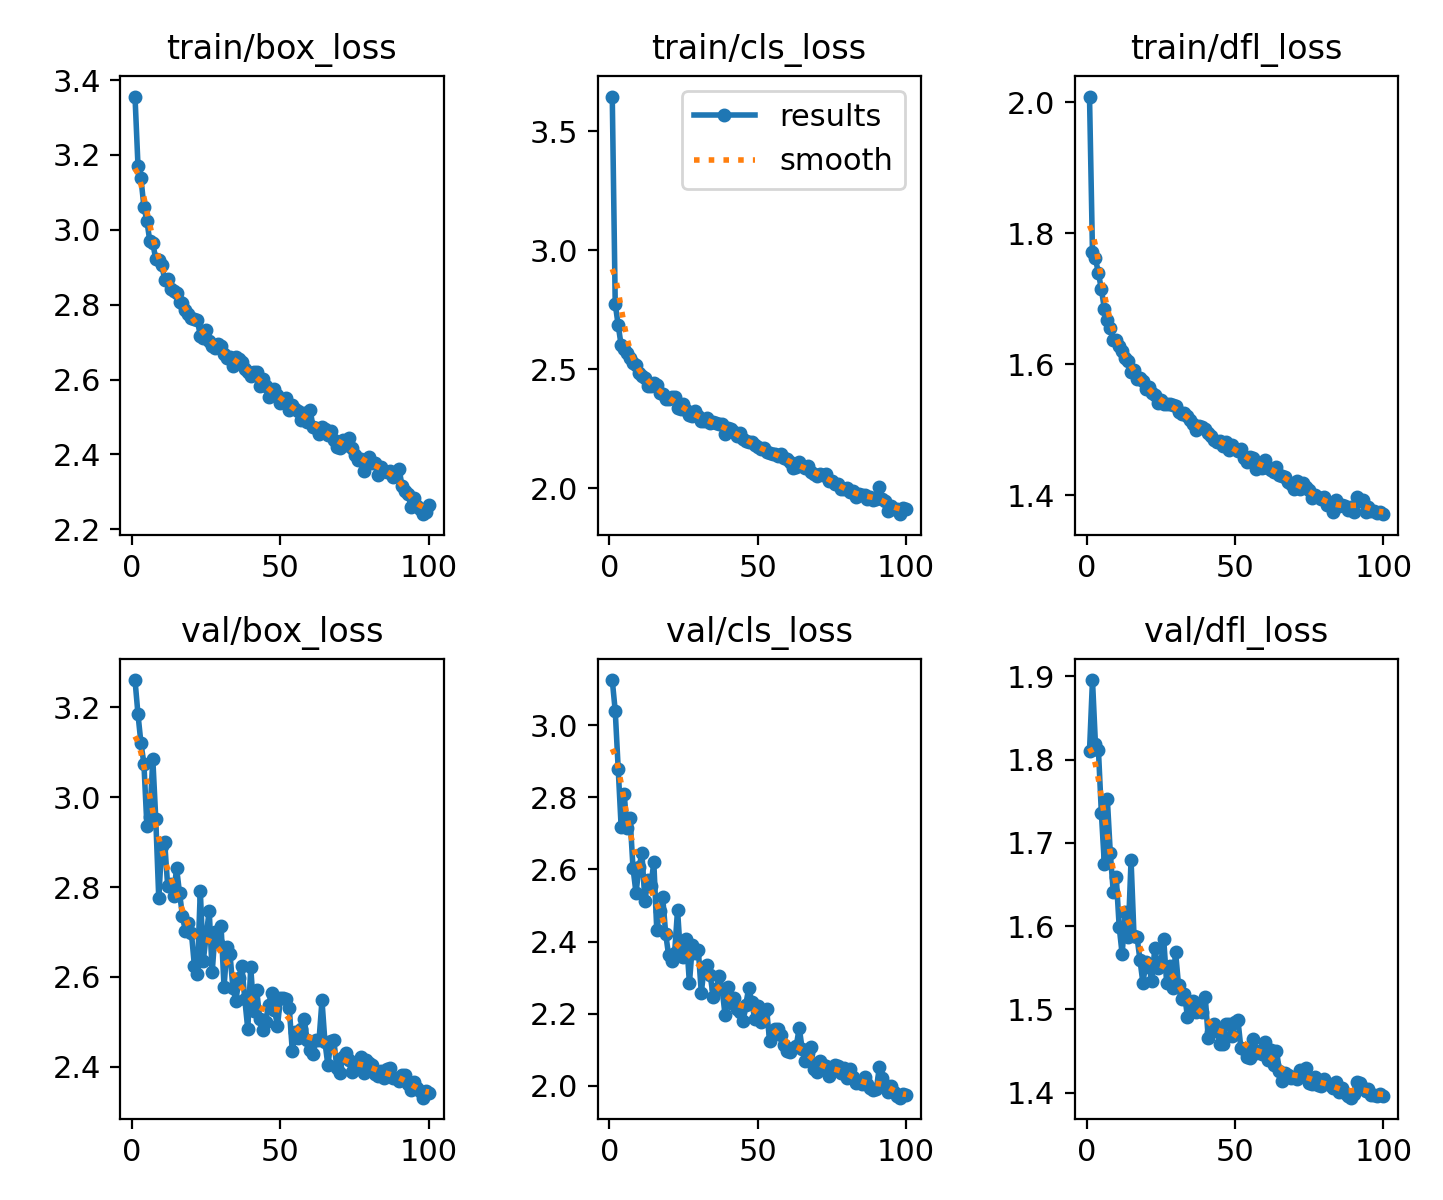
\includegraphics[width=0.95\linewidth]{imageswithoutzero/results(1)copy.png}
    \caption{Training and validation loss curves over 100 epochs for the YOLOv8n
    model trained on the reduced dataset (impact crater class excluded), showing
    box loss, classification loss, and distribution focal loss (DFL).}
    \label{fig:loss_reduced}
\end{figure}

\begin{figure}[htbp!]
    \centering
    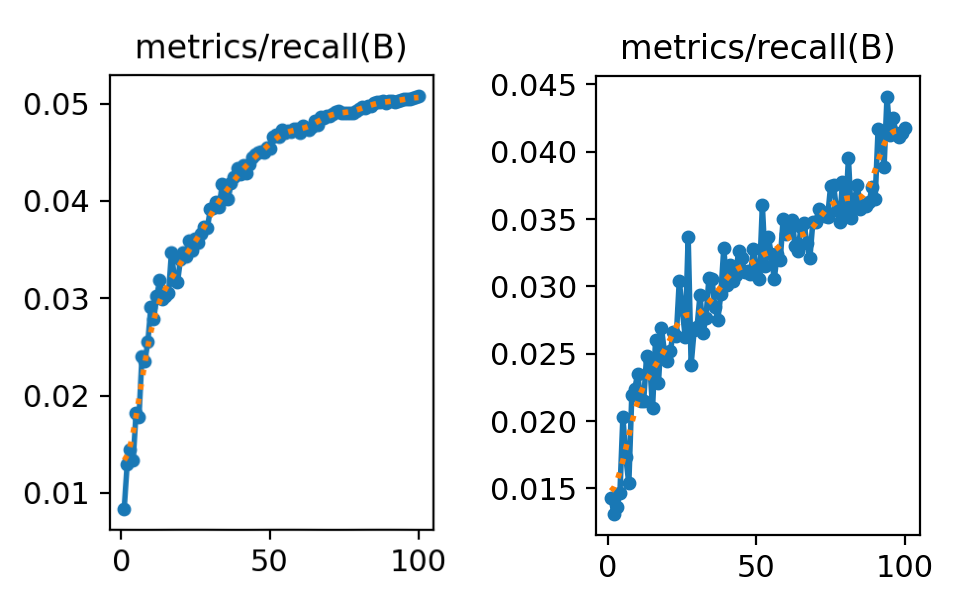
\includegraphics[width=\linewidth]{./image.png}
    \caption{Recall curves over 100 training epochs for both
    experiments. Right: full dataset --- recall grows slowly to $\sim$0.05,
    reflecting the dominance of the impact crater class. Left: reduced
    dataset --- recall grows steadily to $\sim$0.043, now spread across the
    six rare classes rather than concentrated on craters.}
    \label{fig:metrics_comparison}
\end{figure}

\section{South pole: inference diagnostics and the defective run}
\label{app:southpole}

Figure~\ref{fig:south_pole_diag} shows the per-class confidence diagnostics behind Table~\ref{tab:south_pole_stats}, and Fig.~\ref{fig:south_pole_best} the best-detected tile per class. Figure~\ref{fig:mega_grid_3x2} documents the defective pipeline run analysed in Sect.~\ref{sec:southpole}.

\begin{figure*}[htbp]
\centering
\begin{subfigure}[b]{0.48\textwidth}
    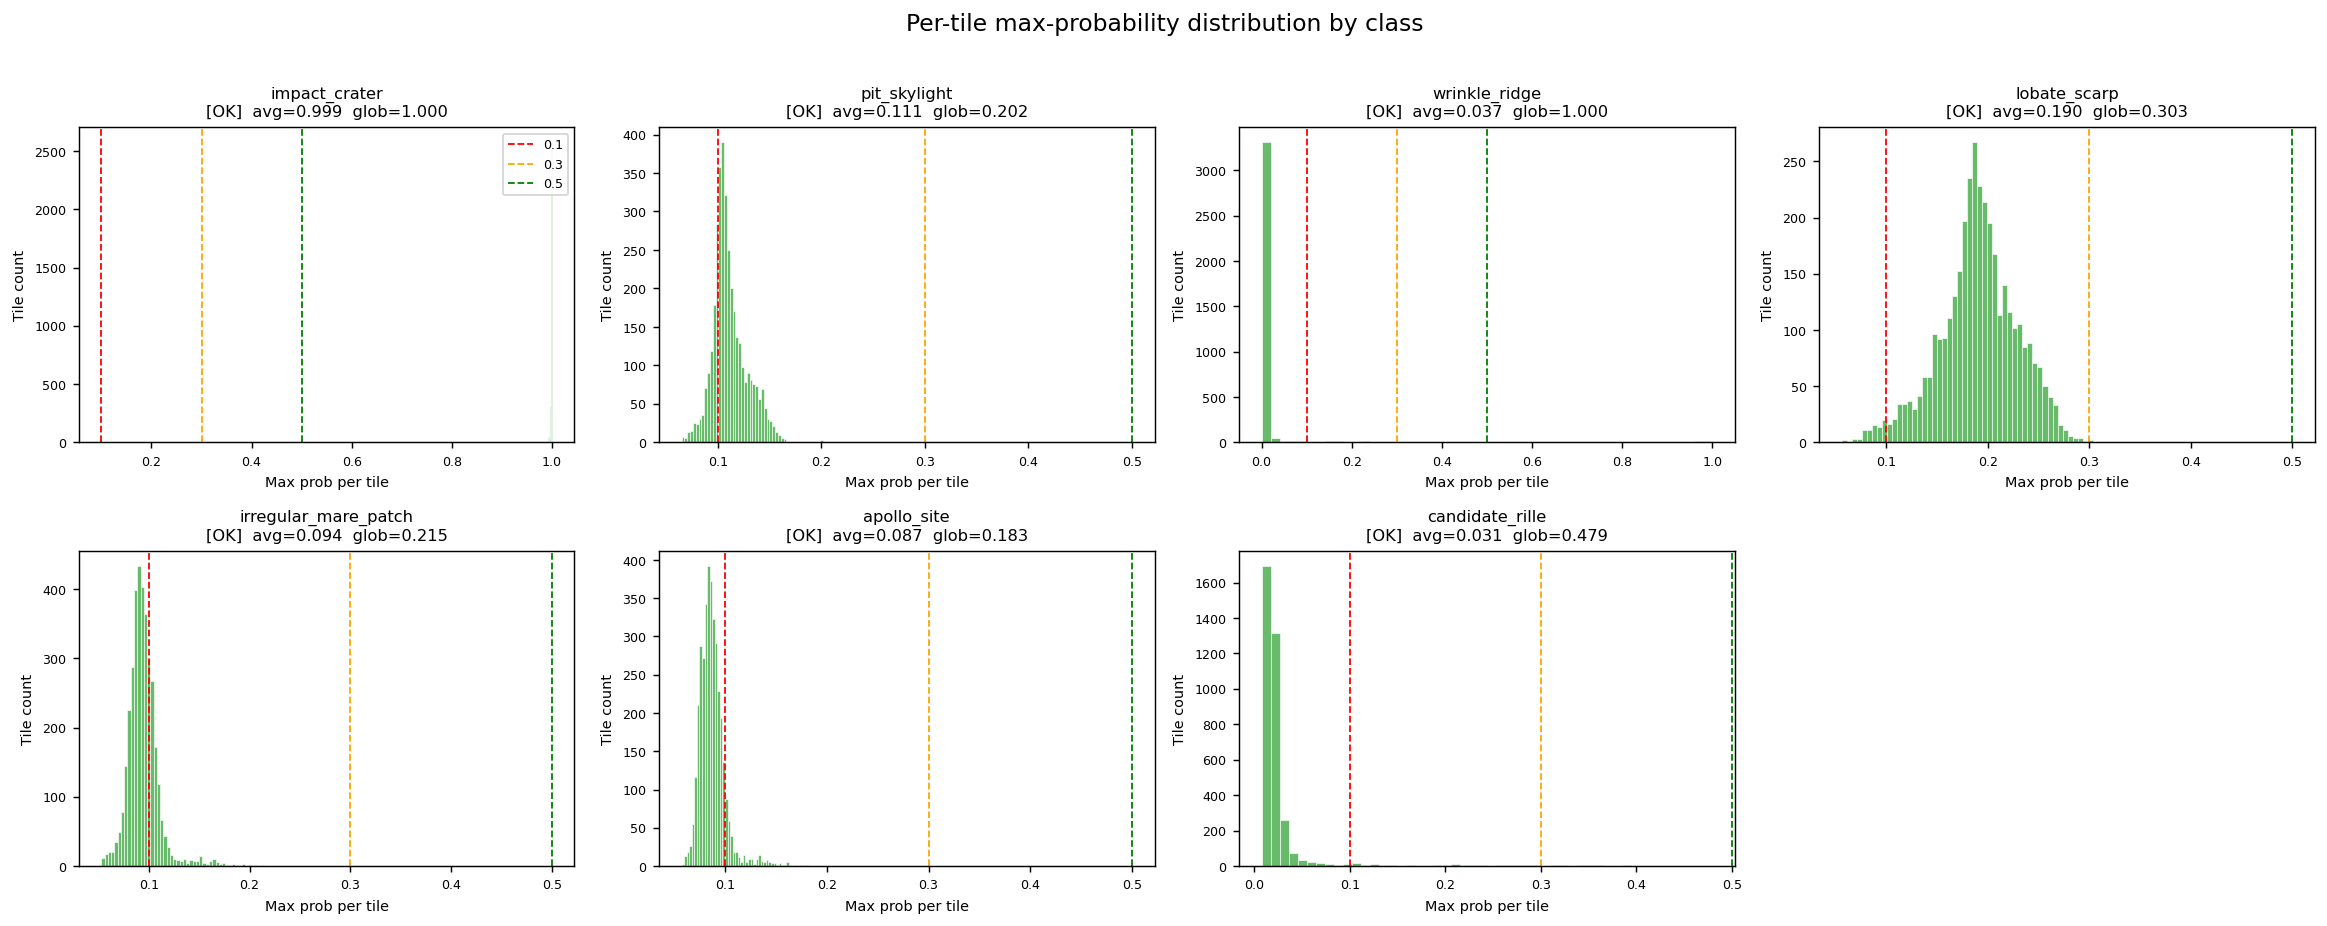
\includegraphics[width=\textwidth]{figures/MR/diagnostics_distributions.png}
    \caption{Per-tile max-probability distributions.}
\end{subfigure}
\hfill
\begin{subfigure}[b]{0.48\textwidth}
    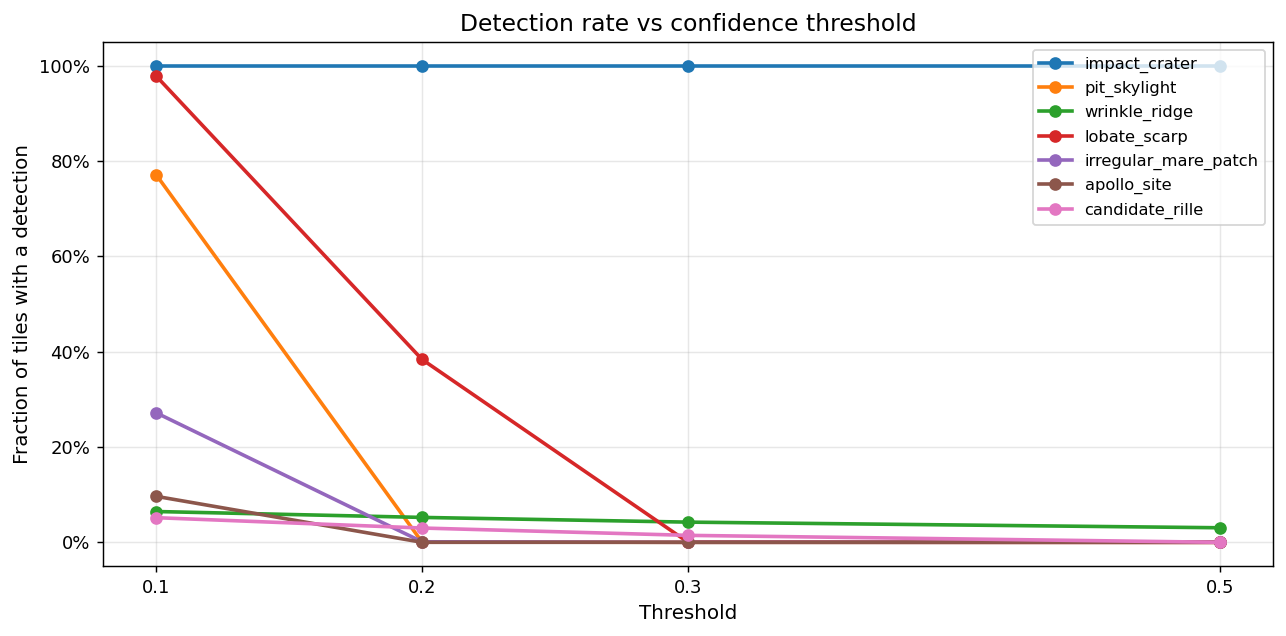
\includegraphics[width=\textwidth]{figures/MR/diagnostics_detection_rates.png}
    \caption{Detection rate vs.\ confidence threshold.}
\end{subfigure}
\caption{South pole inference diagnostics across 3\,639 tiles. Impact craters are detected with near-certainty across the entire region. All other classes exhibit strongly right-skewed distributions with low average confidence, reflecting both the domain shift from Marius Hills and the scarcity of these features at the south pole.}
\label{fig:south_pole_diag}
\end{figure*}

\begin{figure}[htbp!]
\centering
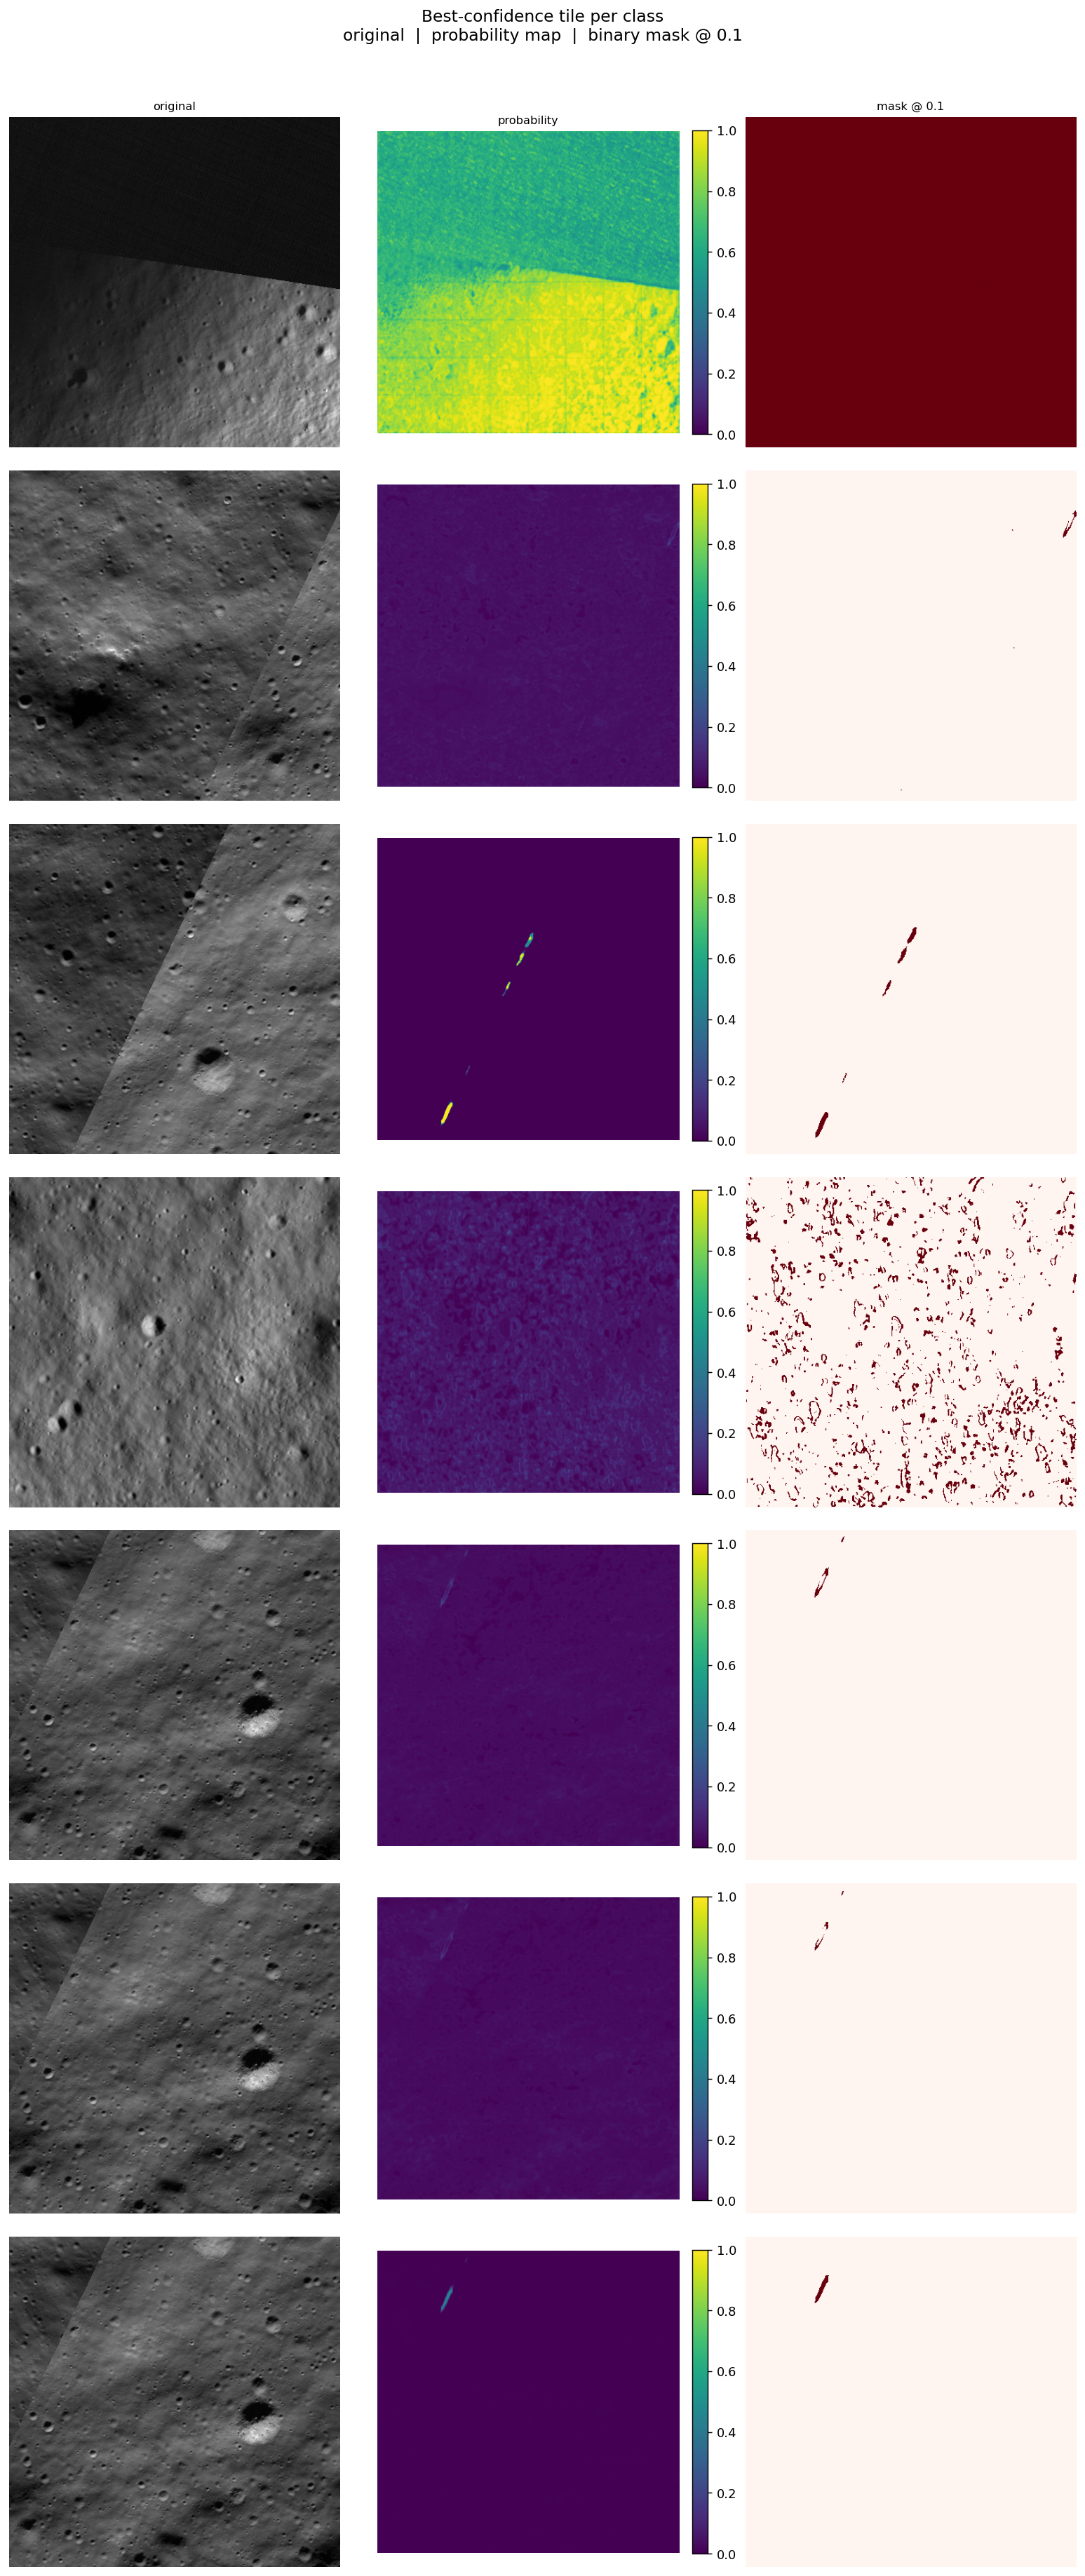
\includegraphics[width=0.85\columnwidth,keepaspectratio]{figures/MR/diagnostics_best_tiles.png}
\caption{Best-detected tile per class on the south pole imagery. Each panel shows the LRO WAC tile overlaid with the predicted probability map for the class with the highest maximum confidence in that tile. Overlays use a \emph{relative} threshold (top fraction of each tile's probabilities), so coloured regions for the weak classes are candidate locations, not confident detections.}
\label{fig:south_pole_best}
\end{figure}

\begin{figure*}[htbp]
\centering
  \begin{subfigure}[b]{0.4\textwidth}
    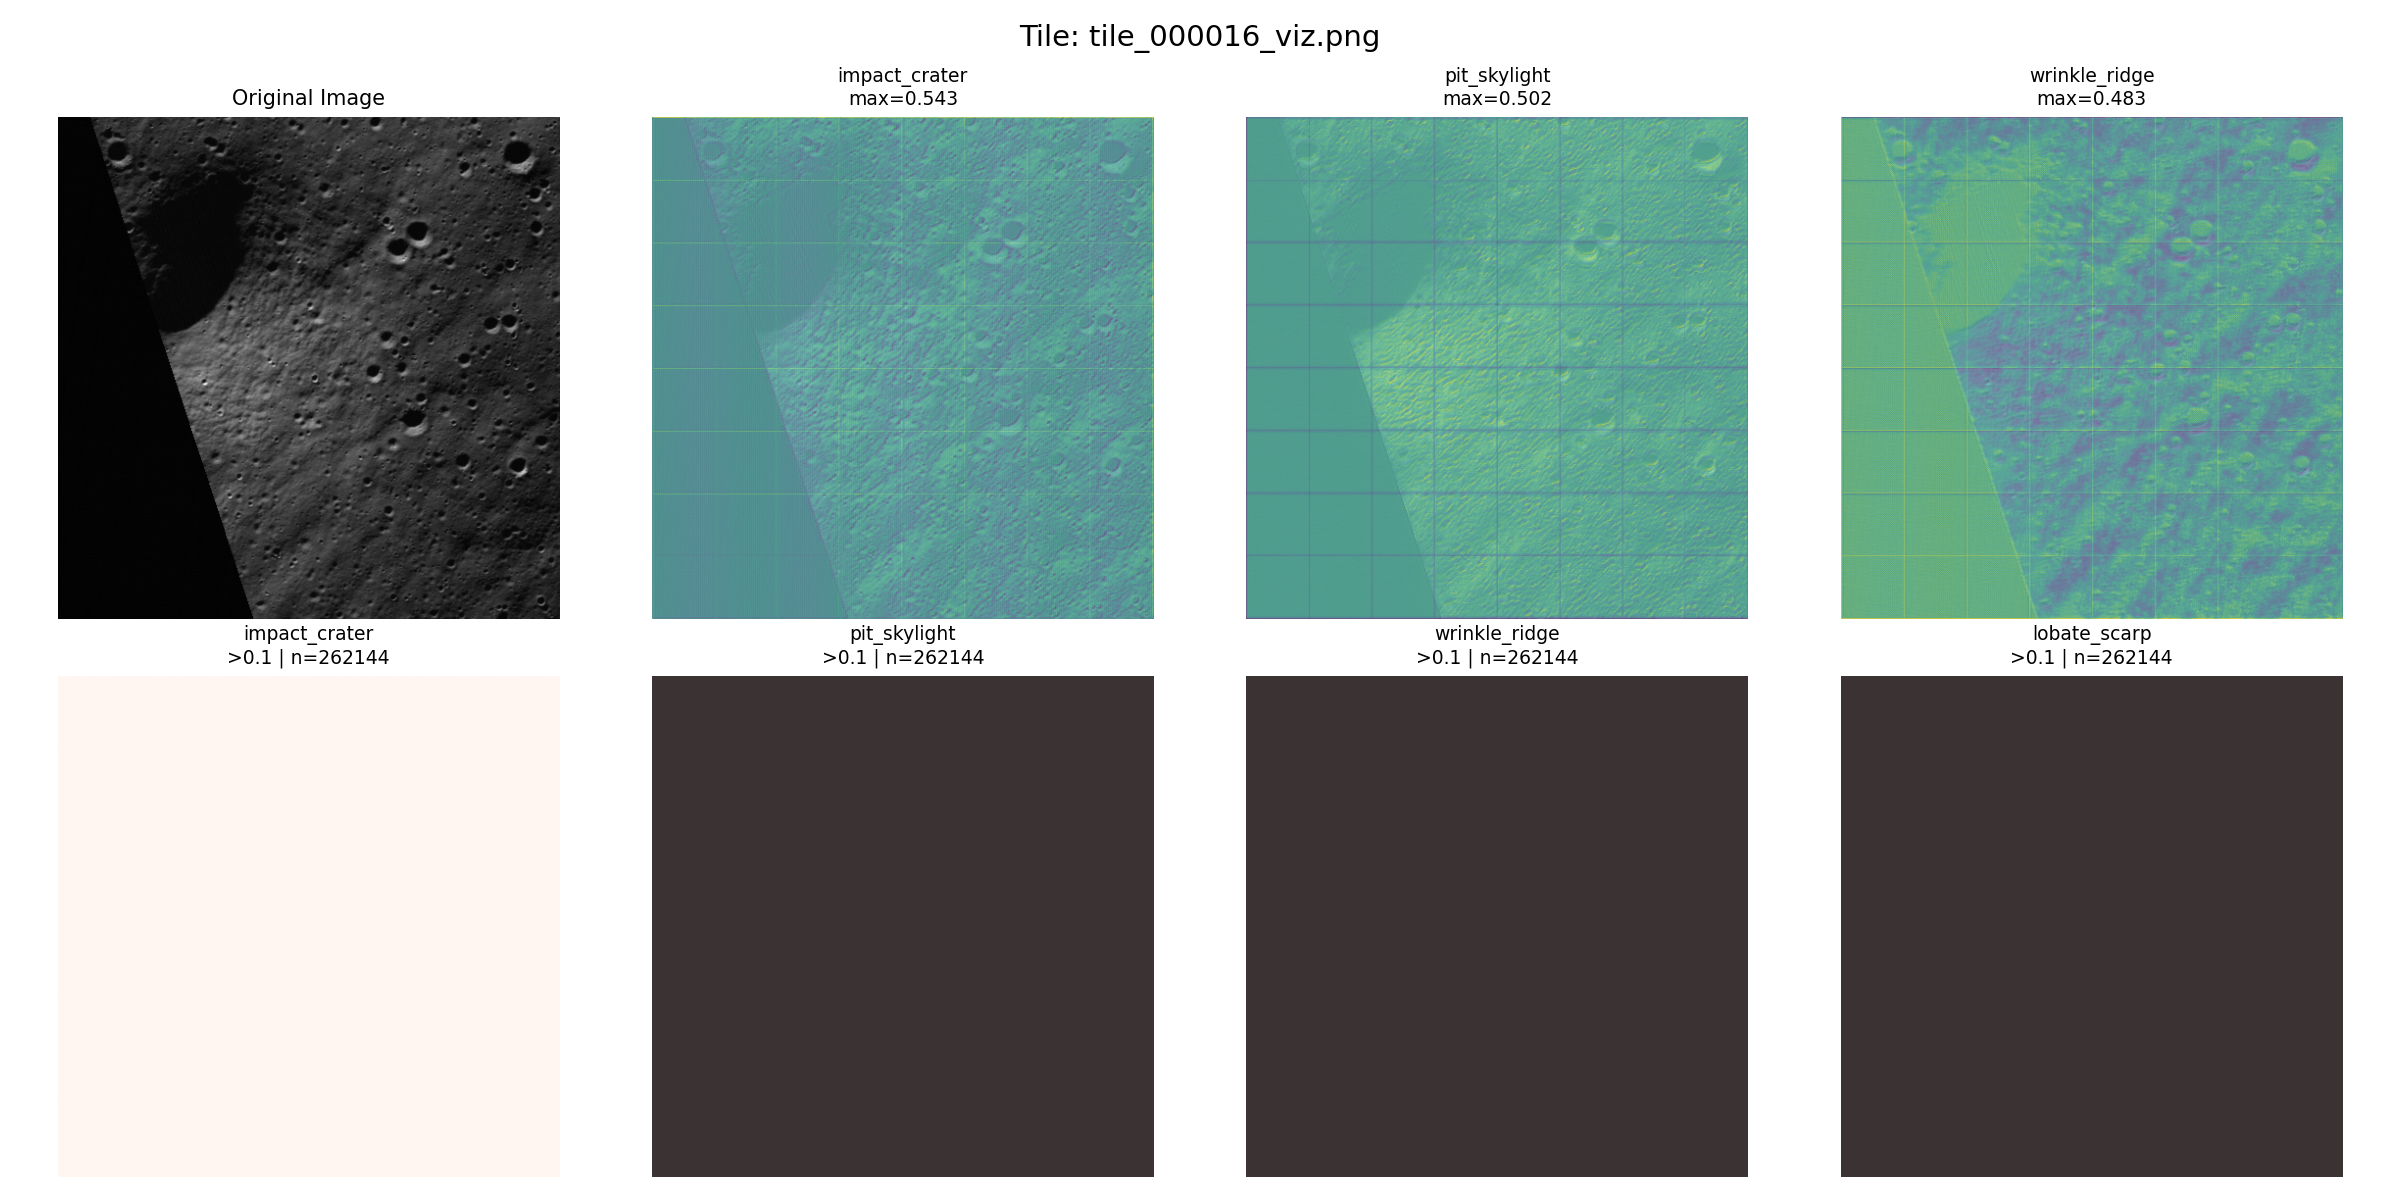
\includegraphics[width=\textwidth]{output1.png}
    \caption{Tile 1.}
  \end{subfigure}
  \hfill
  \begin{subfigure}[b]{0.4\textwidth}
    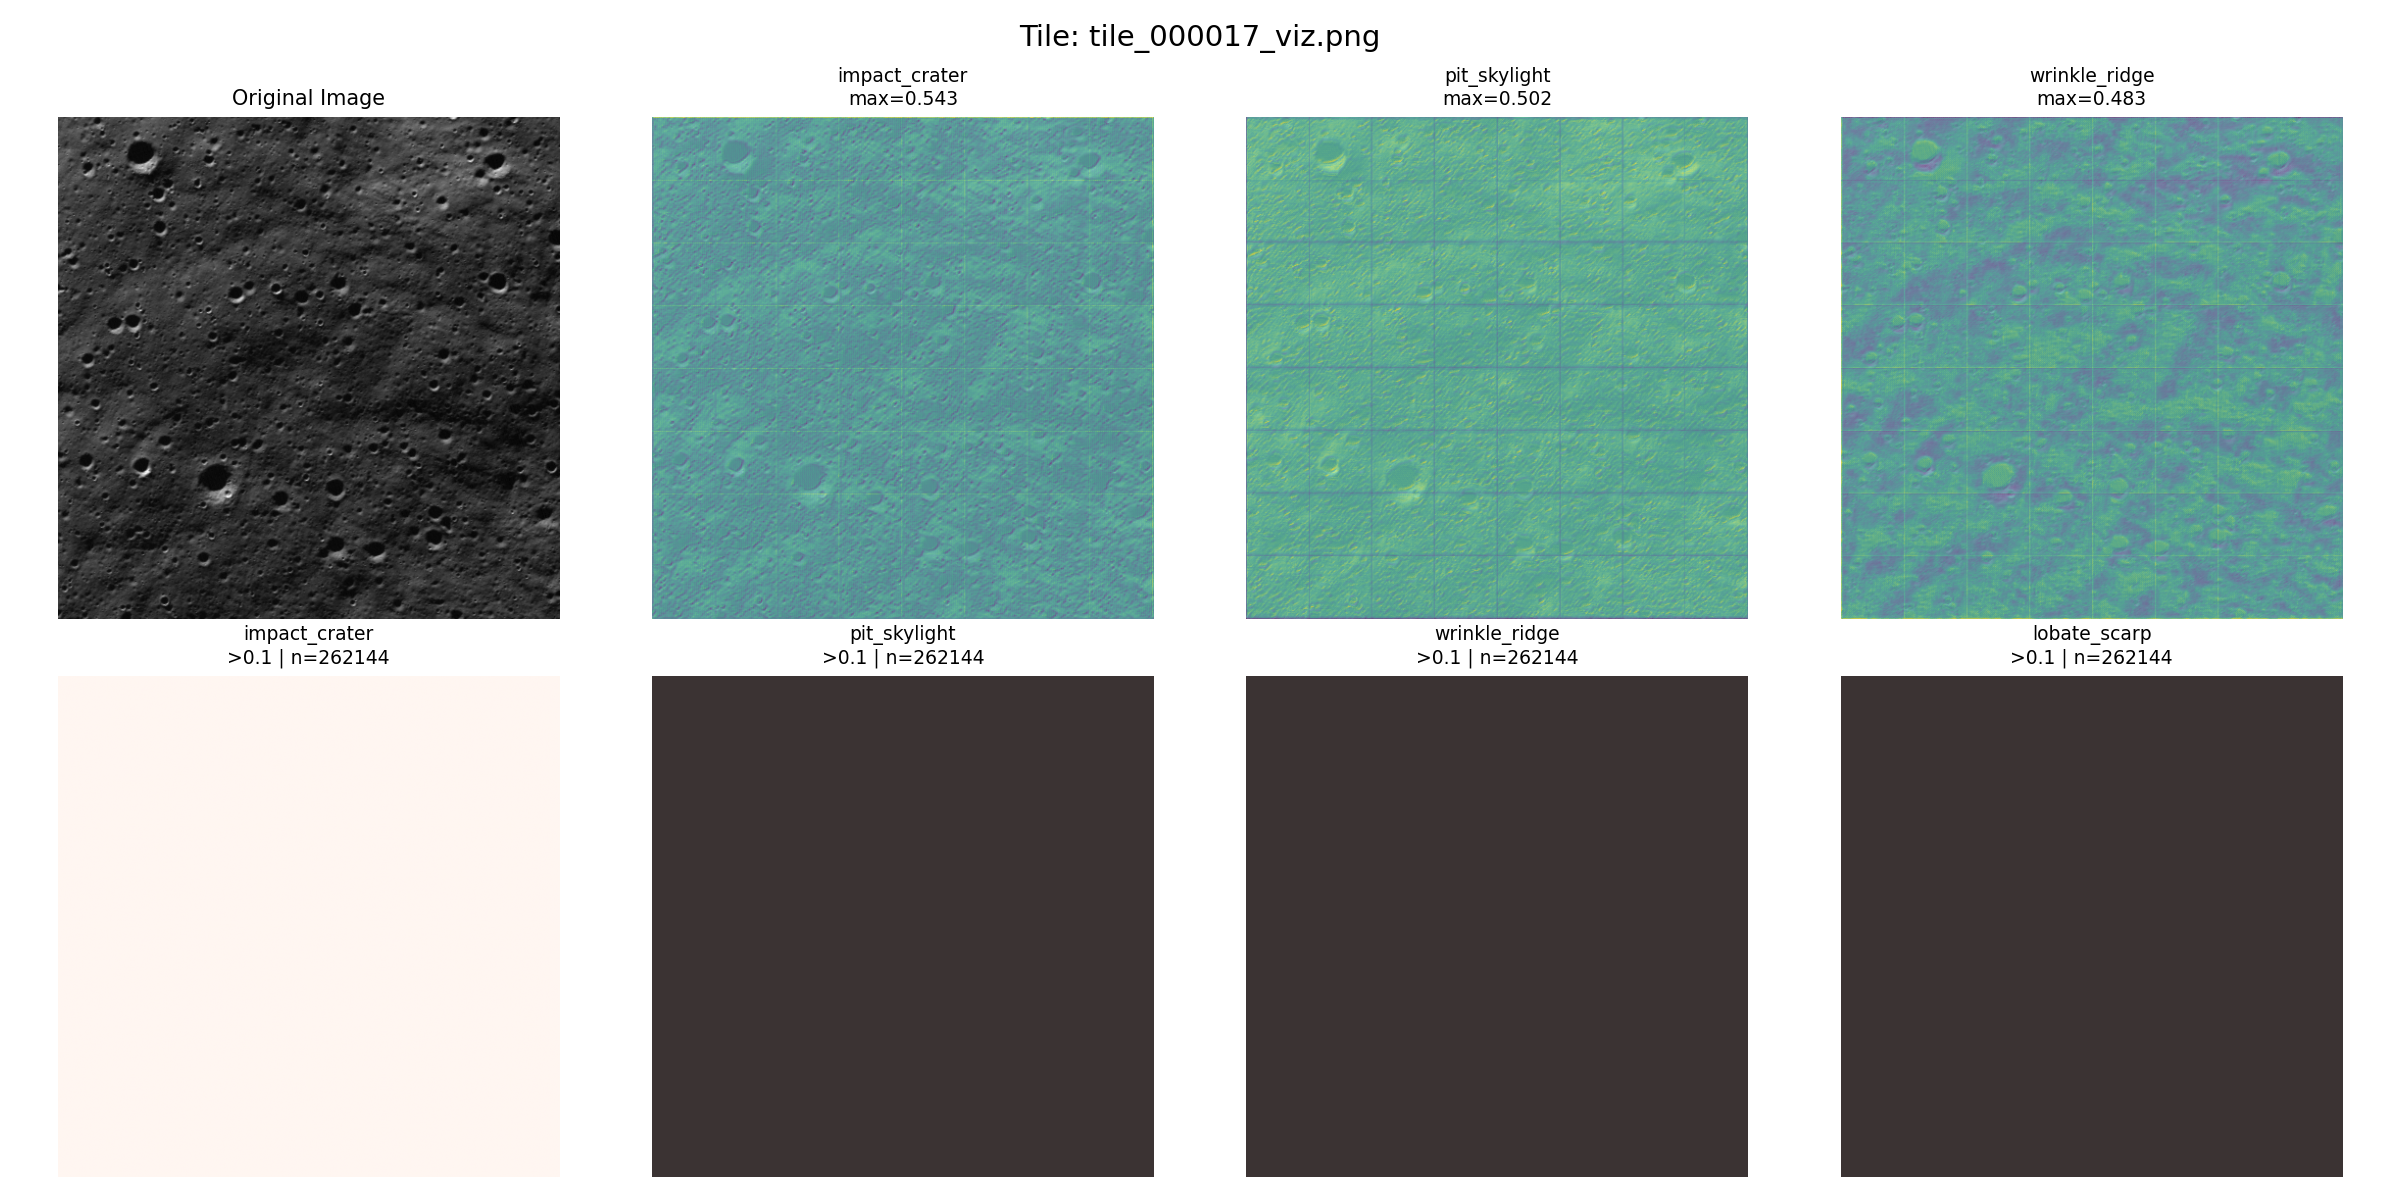
\includegraphics[width=\textwidth]{output2.png}
    \caption{Tile 2.}
  \end{subfigure}
  \hfill
  \begin{subfigure}[b]{0.4\textwidth}
    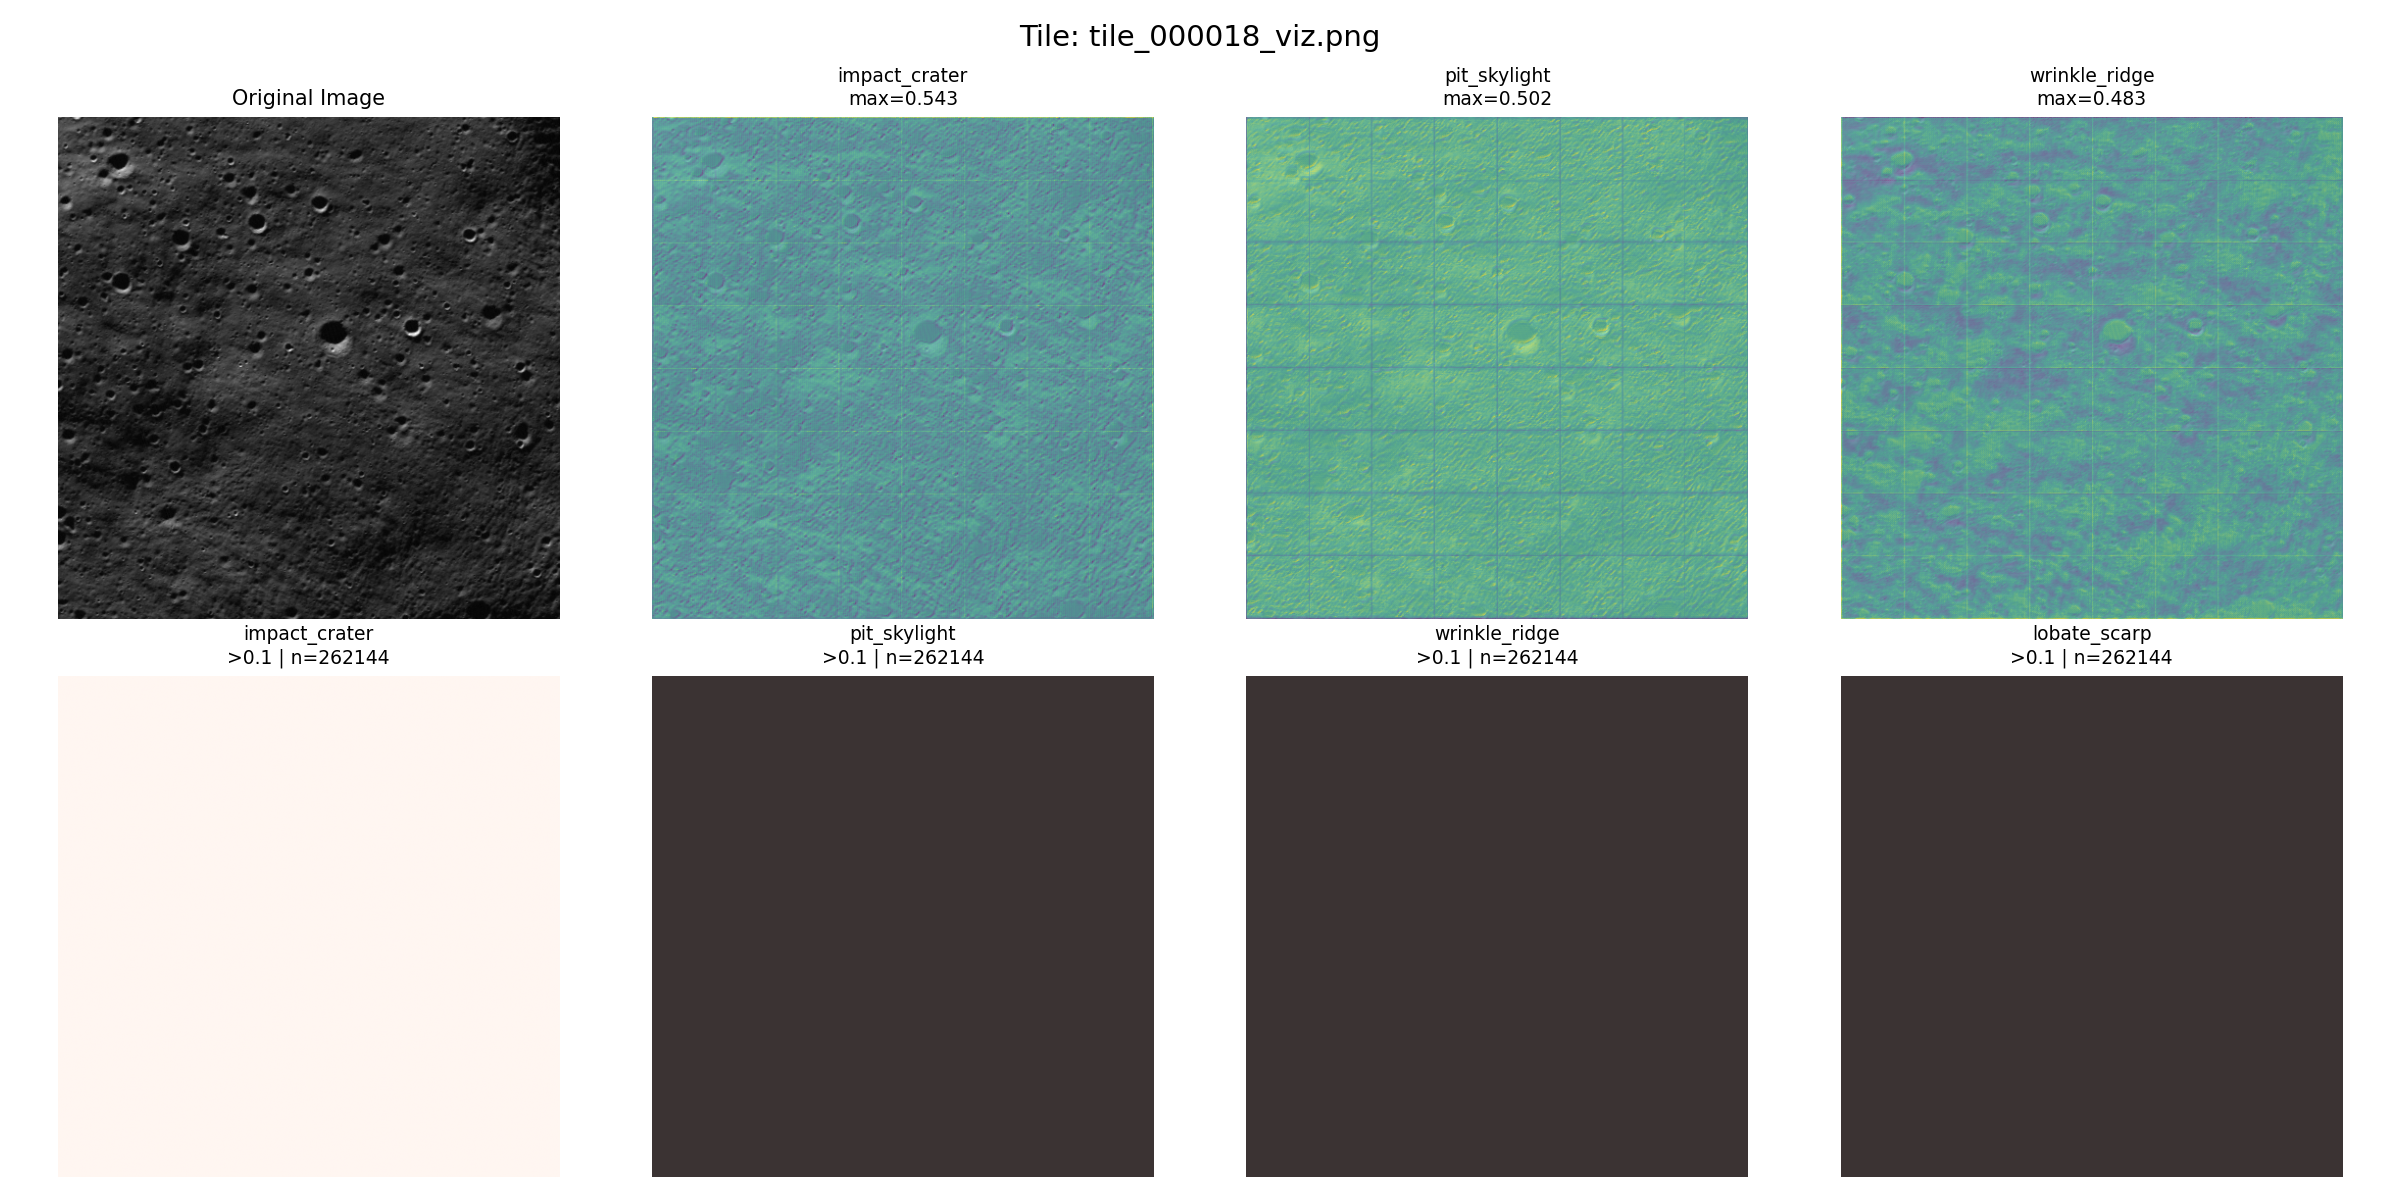
\includegraphics[width=\textwidth]{output3.png}
    \caption{Tile 3.}
  \end{subfigure}

  \vspace{0.5cm}
  \begin{subfigure}[b]{0.4\textwidth}
    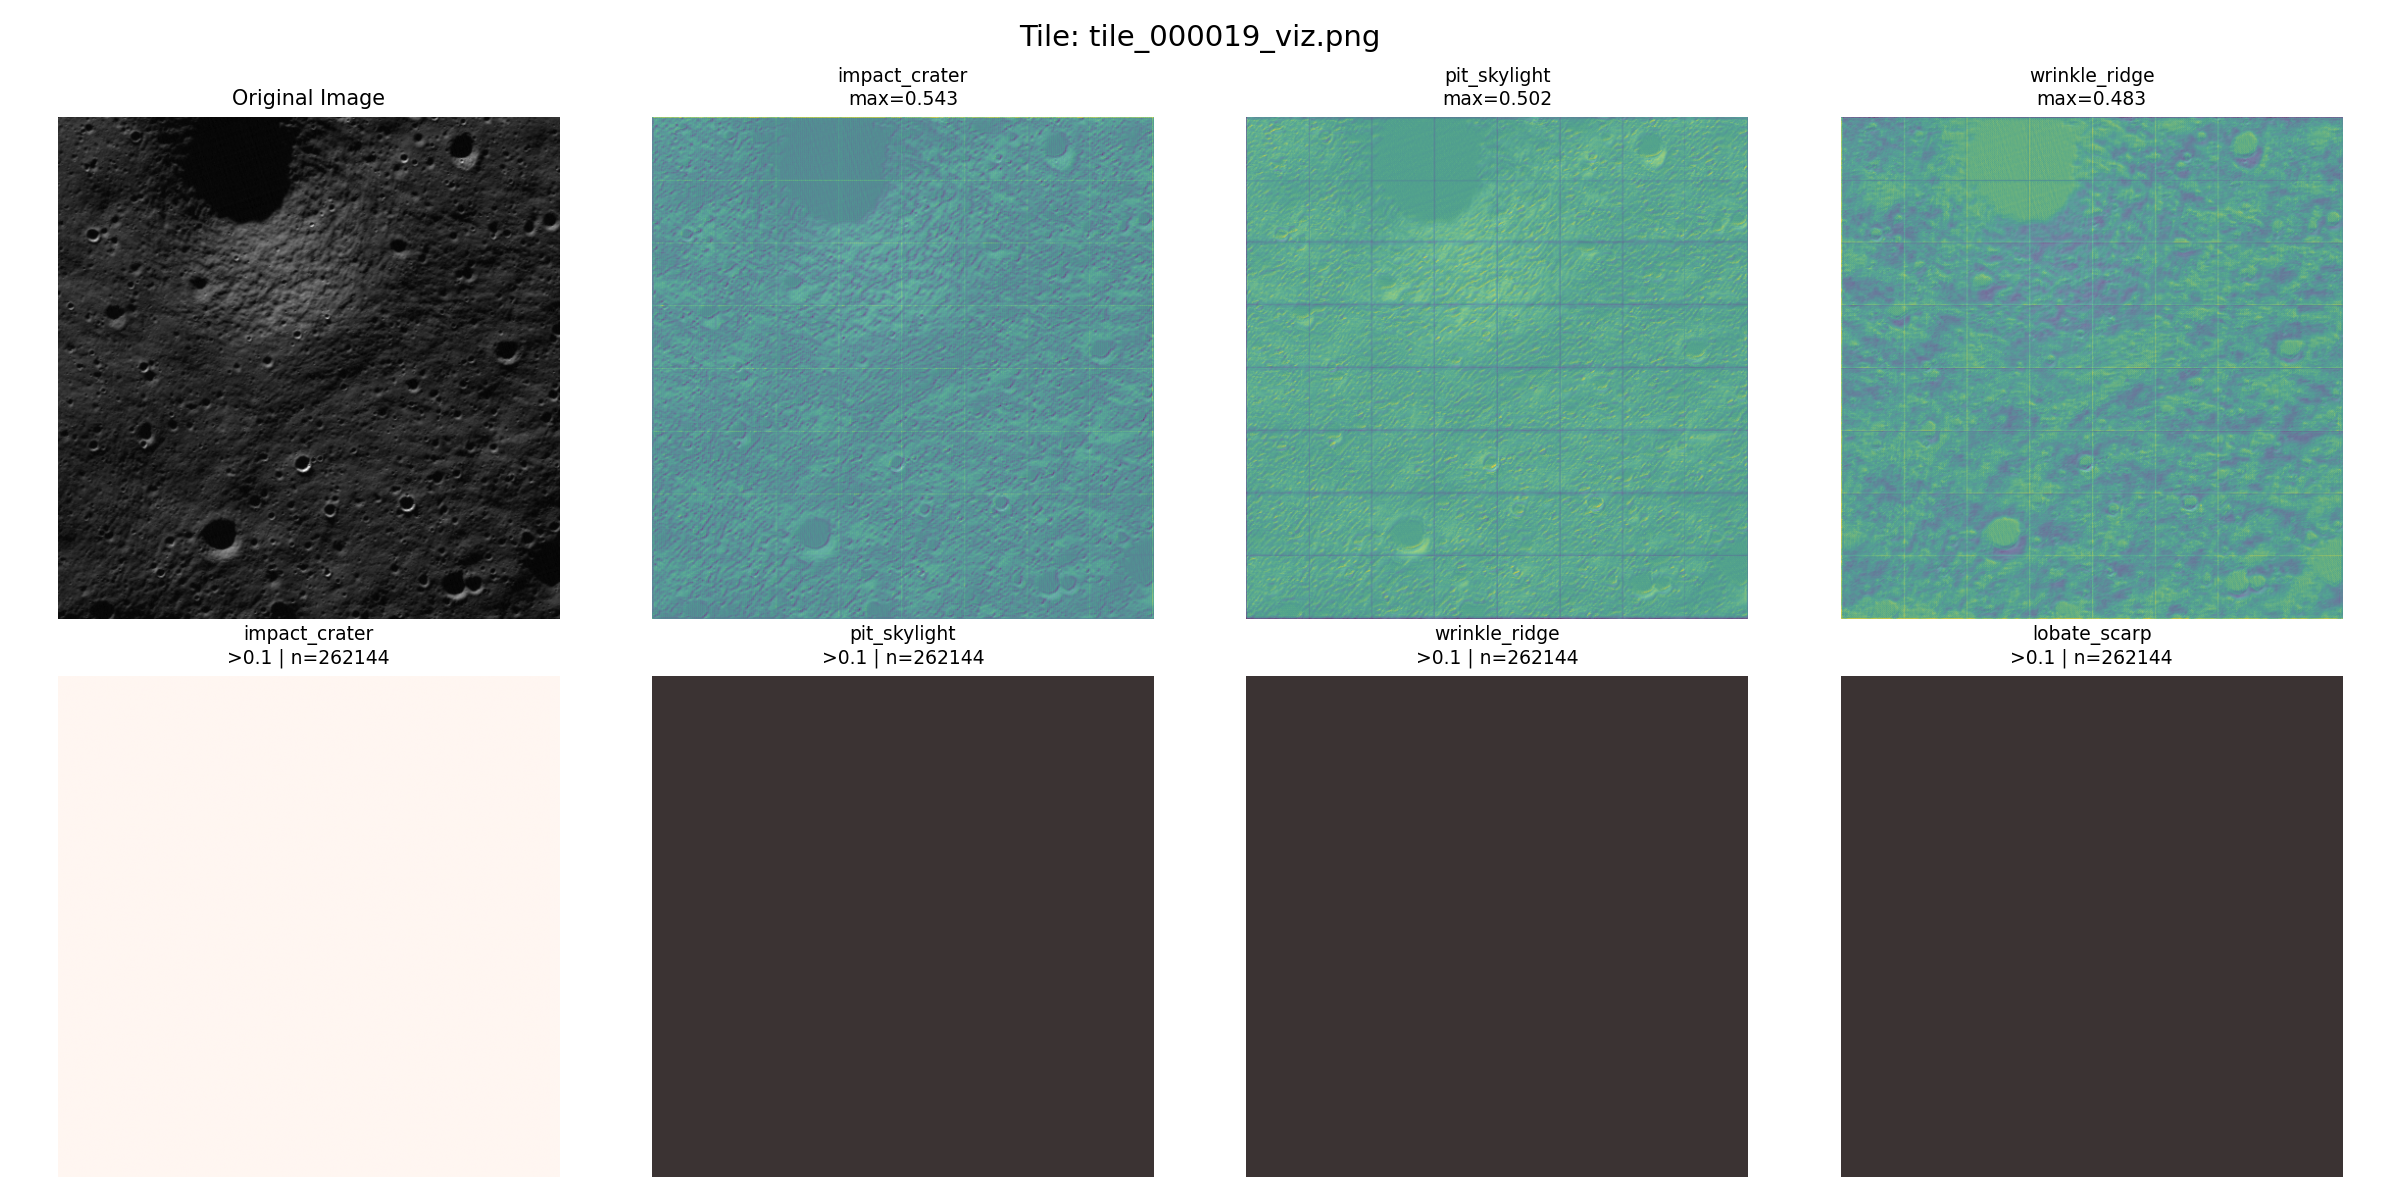
\includegraphics[width=\textwidth]{output4.png}
    \caption{Tile 4.}
  \end{subfigure}
  \hfill
  \begin{subfigure}[b]{0.4\textwidth}
    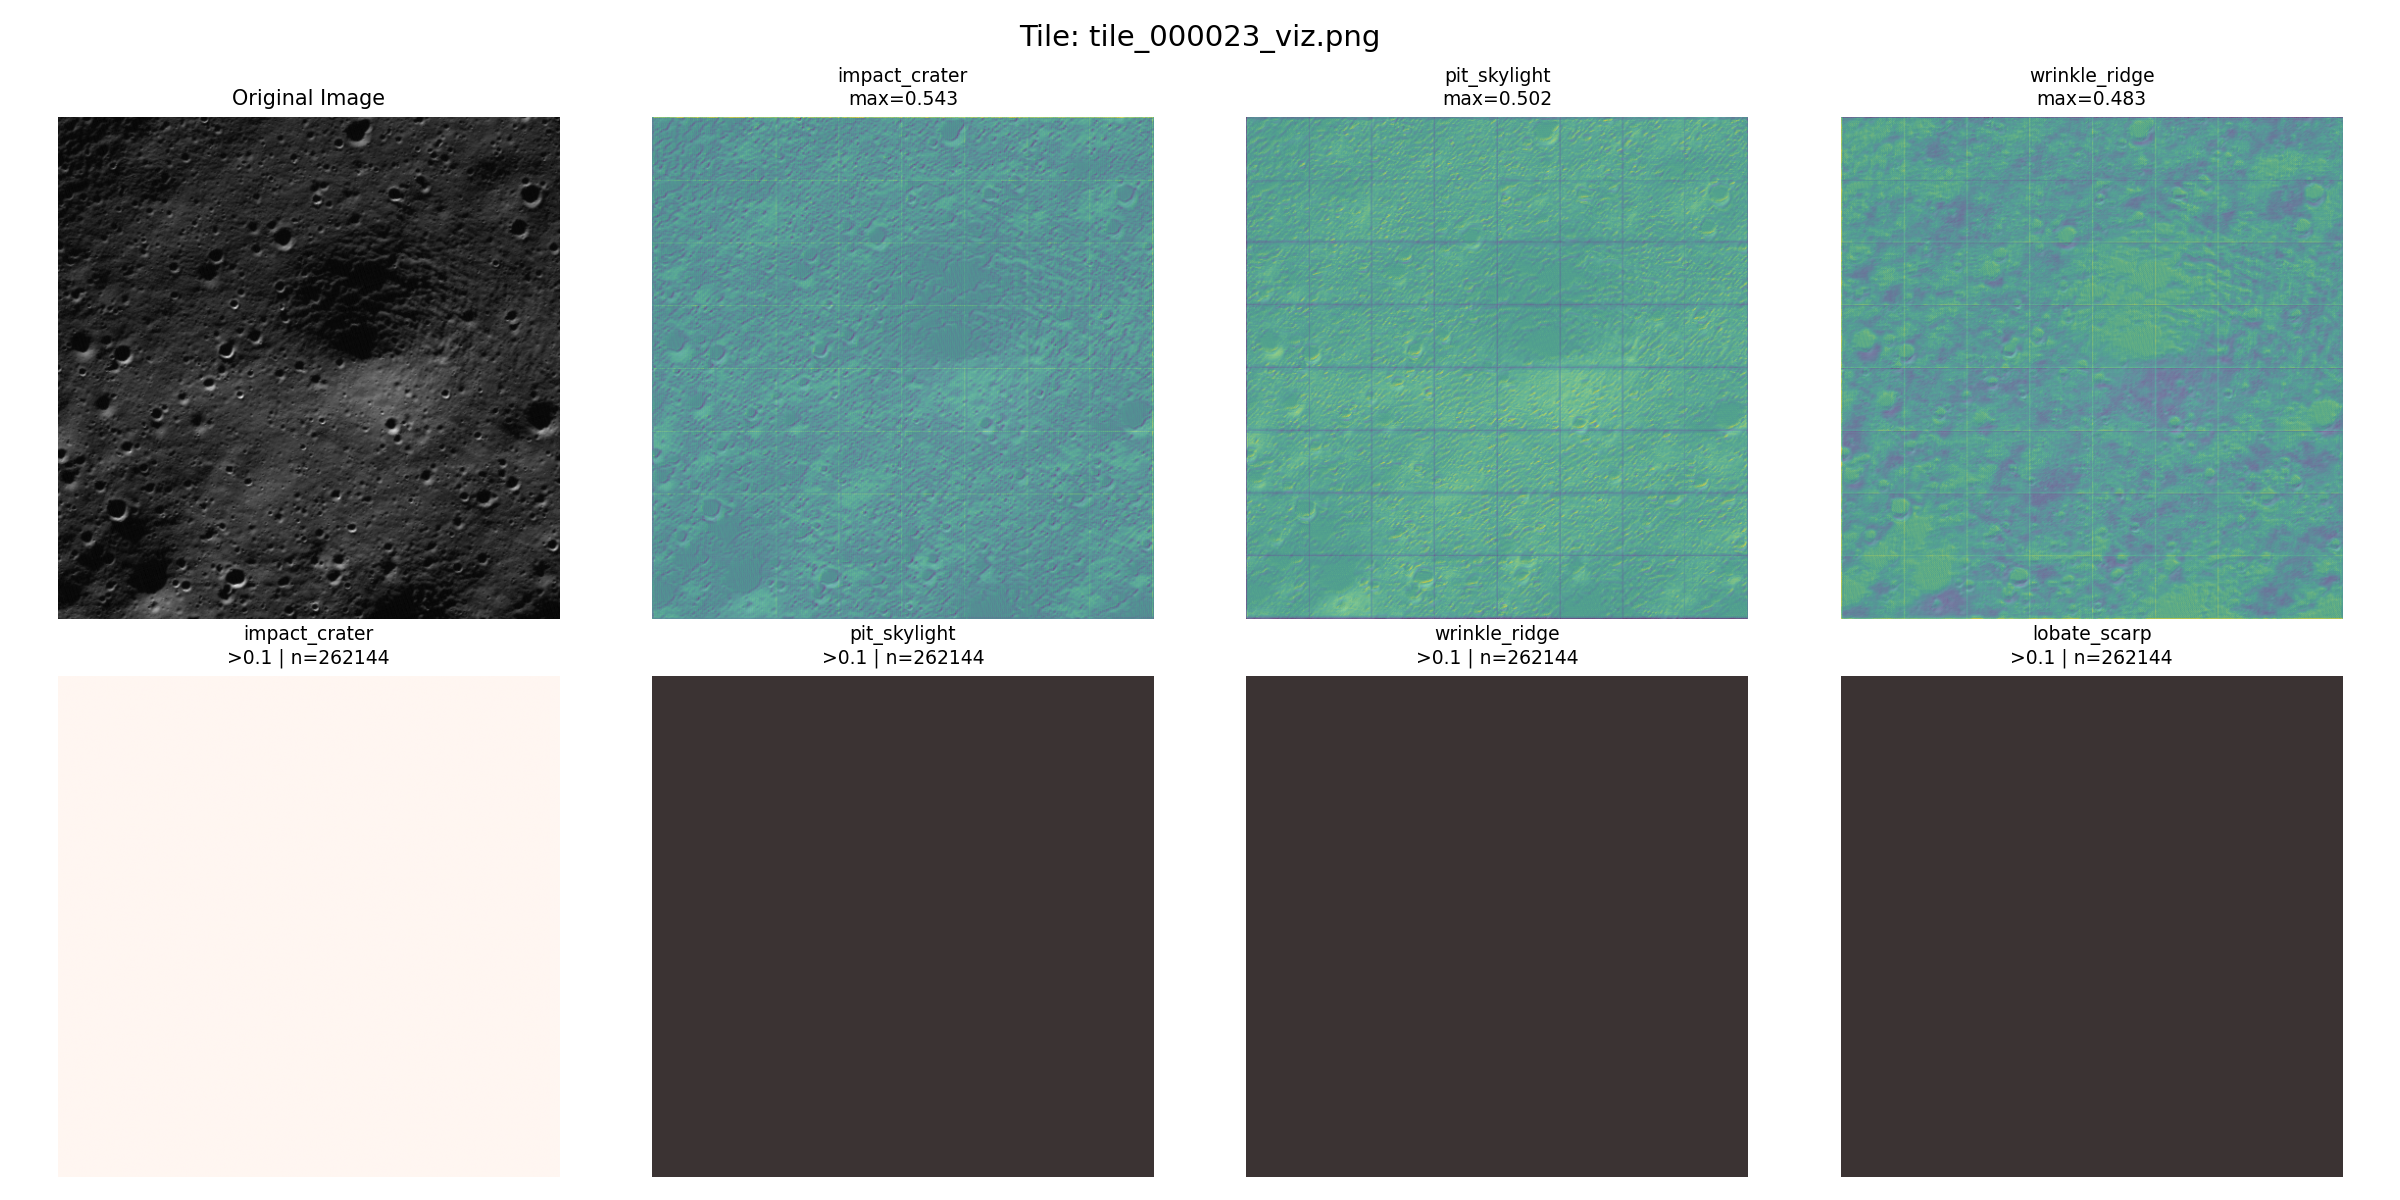
\includegraphics[width=\textwidth]{output5.png}
    \caption{Tile 5.}
  \end{subfigure}
  \hfill
  \begin{subfigure}[b]{0.4\textwidth}
    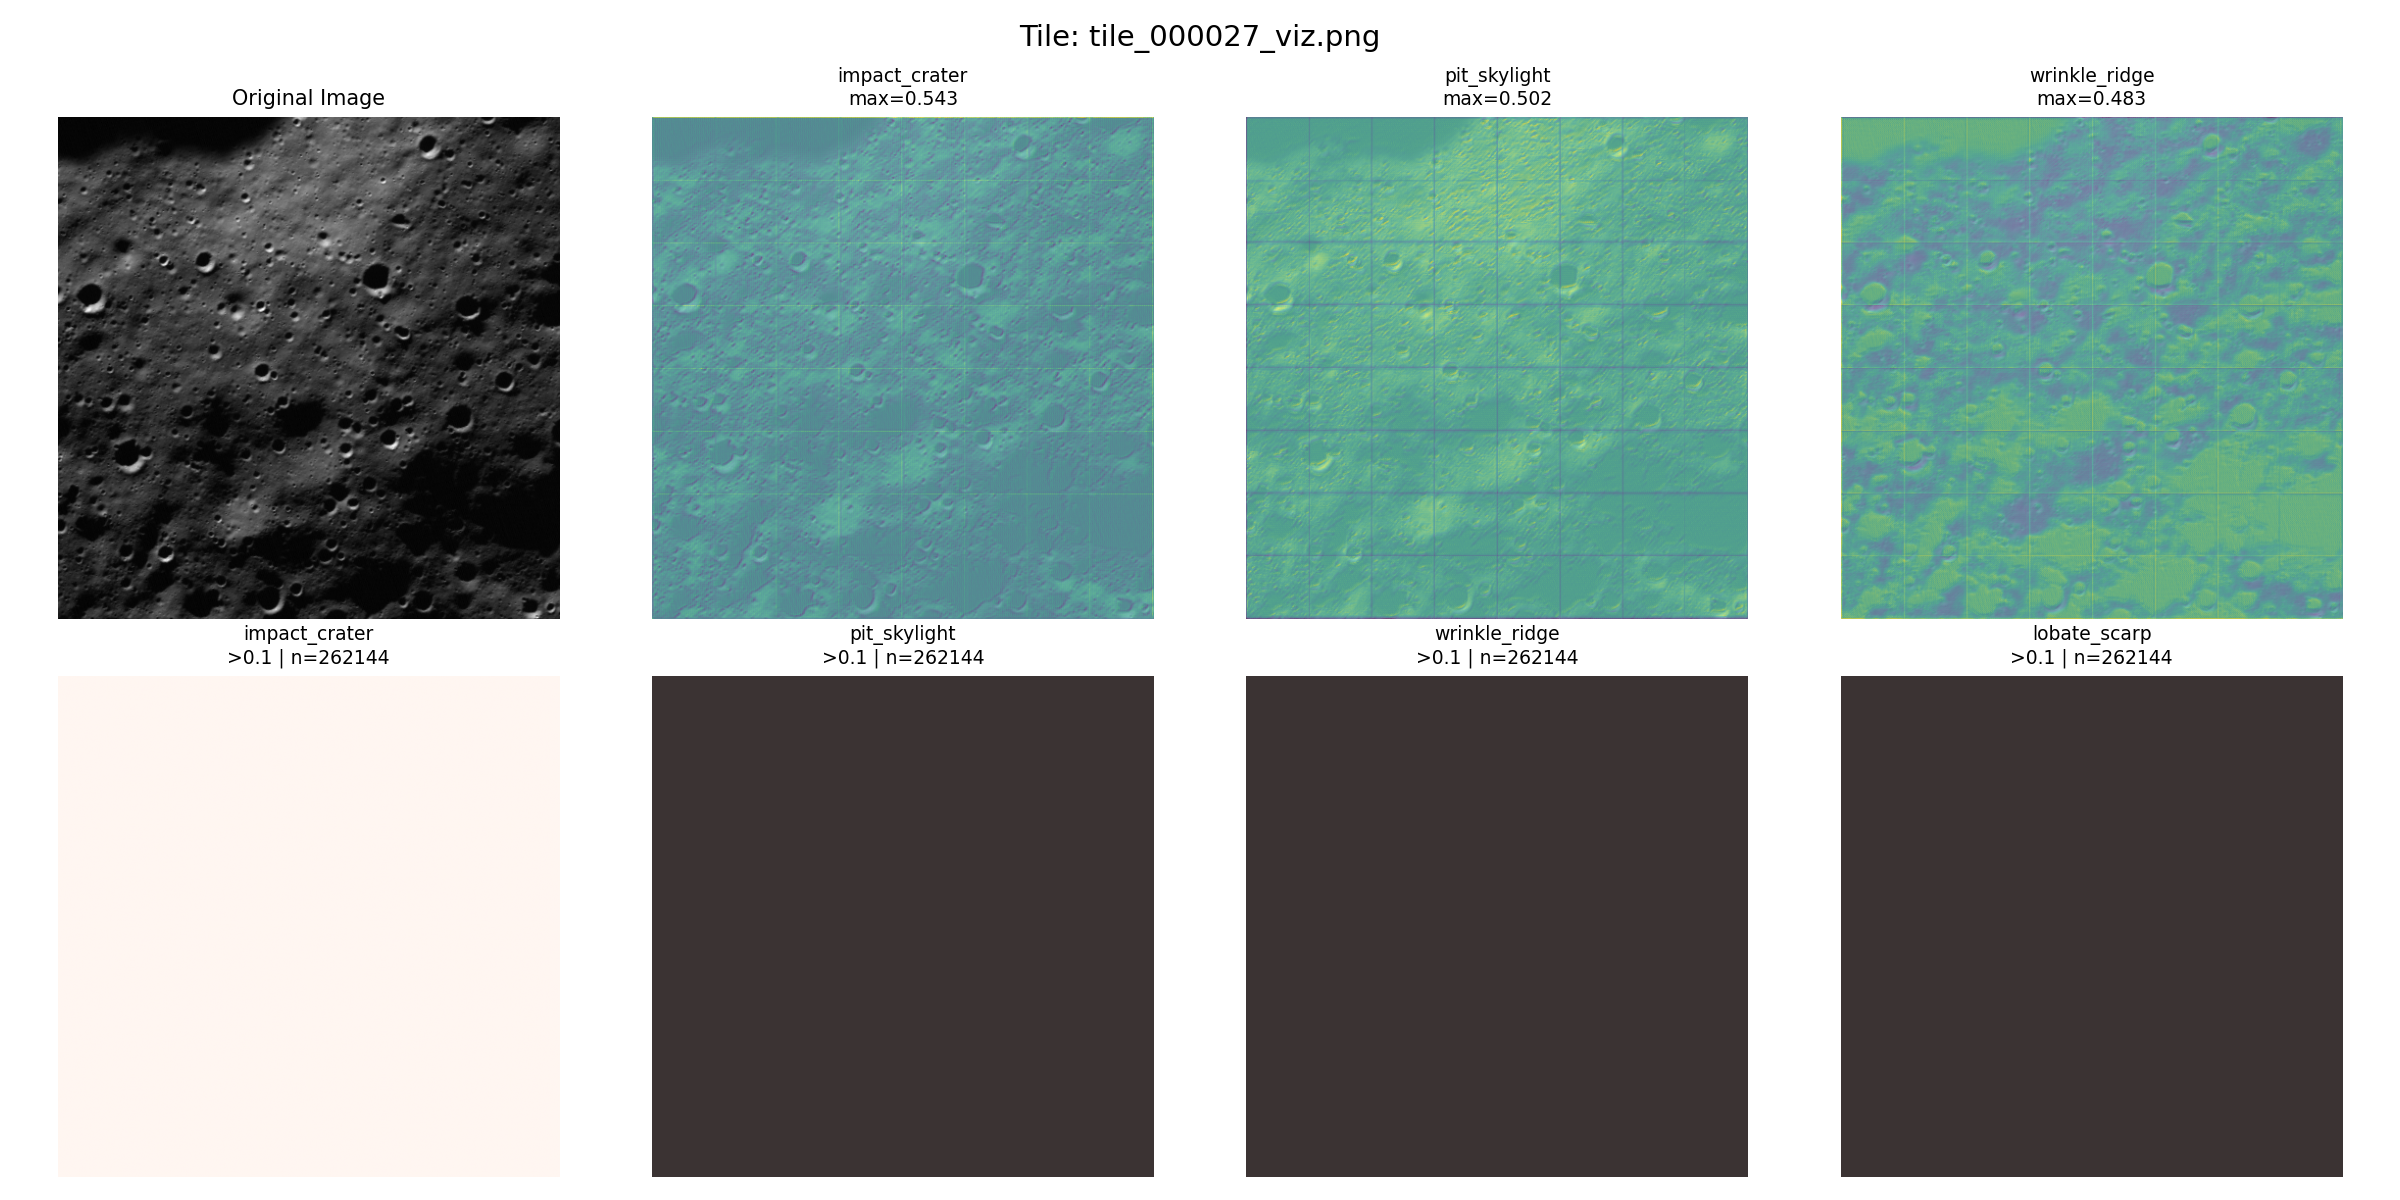
\includegraphics[width=\textwidth]{output6.png}
    \caption{Tile 6.}
  \end{subfigure}

\caption{Visual-verification outputs of the \emph{initial, defective} pipeline run on six south pole tiles (original imagery alongside per-class probability overlays). The overlays are flat and near-uniform regardless of the underlying morphology --- the visual signature of the silently unmatched checkpoint described in Sect.~\ref{sec:southpole}: a randomly initialised network outputs $\approx0.5$ everywhere, which post-processing renders as structureless fields. The corrected pipeline instead reproduces the class-selective behaviour of Table~\ref{tab:south_pole_stats}. The panels are retained precisely because they show how plausible a defective run can look at a glance.}
\label{fig:mega_grid_3x2}
\end{figure*}

\end{appendix}
